\documentclass[12pt,a4paper,oneside]{article}
\usepackage[total={170mm,250mm}]{geometry}
% Toward automatic robot programming: learning human skill from visual data
\usepackage{graphicx}
\usepackage{multicol}
\usepackage{multirow}
\usepackage[]{natbib}
\usepackage{subfiles}
\usepackage{booktabs}
\usepackage{amsmath}
\usepackage{amssymb}
\usepackage{subcaption}
\usepackage{adjustbox}
\usepackage{array}
\usepackage{caption}

\usepackage{pdflscape}
\usepackage{lineno}
%\linenumbers
\usepackage{hyperref}


\usepackage{authblk}

\usepackage[table]{xcolor}

\usepackage[shortlabels]{enumitem}
\setlist[enumerate]{nosep}

\usepackage{tikz}
\usepackage{pgfplots}
\usetikzlibrary{calc}
\usetikzlibrary{patterns}
\usetikzlibrary{decorations.text}
\usetikzlibrary{shapes,snakes}


\usepackage{subfiles} 
\usepackage{natbib}
\newcommand{\SensorSubSec}[1]{ \vspace{0.5em} \noindent \textit{#1}}

\def\checkmark{\tikz\fill[scale=0.4](0,.35) -- (.25,0) -- (1,.7) -- (.25,.15) -- cycle;} 

\date{\vspace{10ex}}

%
\graphicspath{{./Diagrams/}{./Images/}}
%
\title{From art to part: learning from the traditional smith in developing flexible sheet metal forming processes}


\begin{document}

\author[1]{D.T. Bowen}
\author[2]{I. M. Russo}
\author[2]{C.J. Cleaver}
\author[2]{J.M. Allwood}
\author[1,*]{E.G. Loukaides}
\affil[1]{ Department of Mechanical Engineering, University of Bath}
\affil[2]{ Department of Engineering, University of Cambridge}

%\affil[*]{ corresponding author: e.loukaides@bath.ac.uk}

\maketitle
\vspace{-4cm}
\begin{center}
* corresponding author: e.loukaides@bath.ac.uk
\end{center}
\vspace{1cm}

\begin{abstract}
The traditional metal smith has the remarkable capability to form a variety of part shapes from flat sheets using only a few universal tools. Such versatility is increasingly appealing to manufacturers who now seek to diversify part catalogues and reduce tooling costs. Despite this utility, the laborious, manual nature of these traditional techniques preclude them from meeting modern-day, high-volume demand. Some techniques however, have served as starting points for the development of new flexible metal forming processes, either through automation of the manual process or by developing new processes that closely replicate the traditional techniques. Here, we look closely at some of the techniques used by the traditional smith to form sheets and review automated adaptations of these processes. We find that decision making elements of these adapted processes are not yet as capable as their manual counterparts, suggesting there is still a lot we can learn from the traditional smith. As such, we look both within and beyond the domain of metal forming at the technologies and the methods that can be used to capture the skilled actions of the smith and how the resulting data can be used to enhance the design and operation of mechanised variants. 

\end{abstract}

\newpage

\section{Introduction} \label{sec:intro}

Recent manufacturing trends indicate a return to demand for a more diversified and personalised catalogue of parts, akin to that of the pre-industrial craft production era \citep{Koren2010TheRevolution}. This shift has been noted in the sheet metal forming sector \citep{Lee2012CaseTechnique,Trzepiecinski2020RecentForming} and has subsequently motivated the development of new, more flexible manufacturing processes throughout both industry and academia \citep{Allwood2006AJapan,Yang2018FlexibilityForming}. However, both the design and operation of these new flexible processes can be a challenging and complex task. Acknowledging the versatility and resourcefulness of the traditional metal smith, we look back at the tools and techniques that enabled them to form a diverse range of parts and examine how this body of knowledge can help modern process designers.   

The traditional metal smith was one of many groups of craftsmen described as \textit{``Skilled workers, using general-purpose machines, making exactly what the customer paid for; one product at a time''} \citep{Koren2010TheRevolution}. Working in isolation in small shops, these skilled workers were responsible for the design, manufacture and assembly of relatively simple goods compared with modern products \citep{Groover2015AutomationEdition}.  Using only a small number of tools and techniques, traditional craftsmen were capable of forming a diverse range of parts from initially flat sheets. Crucially, these parts were the product of human effort and skill; they required a combination of manual dexterity and a large number of intuitive, empirical rules derived from an evolved understanding through experience \citep{Hall1961EngineeringRevolution}. 

\begin{figure}[h]
	\centering
	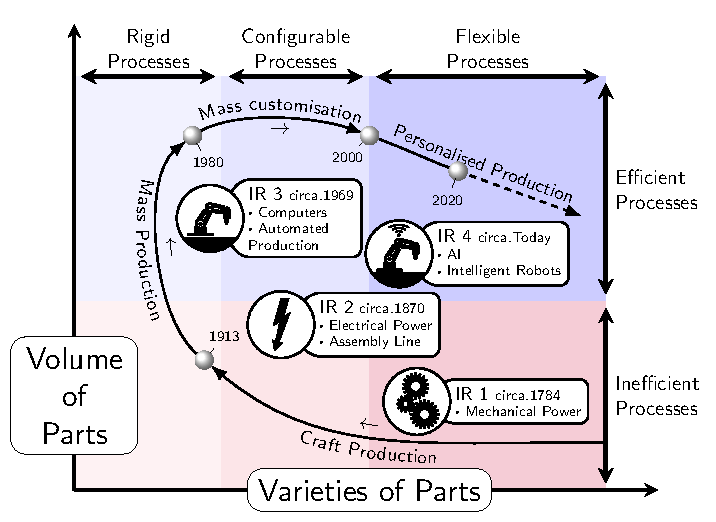
\includegraphics[scale=0.75]{MfgStrat_V6.pdf}
	\caption{Chronological demand for volumes and varieties of parts, subsequent manufacturing paradigms and defining technologies of industrial revolutions (IR), illustrating that the demand for part variety was once obtainable by the craftsman, but has since increased dramatically.}
	\label{fig:VarietyVolume}
\end{figure}

Despite its versatility, the time-consuming and labour-intensive nature of traditional craft production renders it unsuitable for modern-day industrial scale use. This is illustrated in Figure \ref{fig:VarietyVolume} which combines qualitative perspectives from the literature \citep{Koren2010TheRevolution,Popkova2019FundamentalRevolutions,Mourtzis2012DecentralizedOutlook,Mourtzis2014TheCustomisation} to chronologically map changes in market demand over recent centuries. In addition, it shows corresponding manufacturing paradigms and industrial revolutions (IR) whose technology invoked  and/or enabled these shifts in demand. These trends demonstrate how the market is now entering an era of personalised production, requiring high volume production of a high variety of parts. Although traditional techniques developed by the smith have been used in modern-day, high-value, low-volume production of personalised sheet metal parts \citep{Amos2015Bloodhoundfeathers}, their inefficiencies preclude them from meeting modern-day, high-volume demand.

Instead, the requirement for high-volume personalised production within metal forming has motivated development of new, more flexible manufacturing processes throughout both industry and academia \citep{Allwood2006AJapan,Yang2018FlexibilityForming}. These flexible processes are characterised by the ability to produce an extended range of part geometries without the need for part-specific tooling. This provides a more cost effective and sustainable method of meeting these new demands when compared with typical mass-production metal forming processes, which require bespoke tooling and produce substantial waste in the form of discarded materials and workpiece offal, alongside incurred storage and development costs \citep{Cooper2017TheProcesses,Horton2019ImplementingComponents}. 

%The design of hardware and suitable control logic for flexible metal forming systems is a topical but challenging task. Due to the stochastic and non-linear nature of the material properties, conventional processes typically require complex control systems, advanced planning and closed-loop control to achieve high quality singular part forms \citep{Allwood2016Closed-loopForming, Tekkaya2015MetalProperties, Polyblank2014Closed-loopProspectus}. The additional degrees of freedom of flexible systems exacerbates these problems. One solution to the issue of flexible process design is look back to the versatile manual techniques used by the metal smith (bottom right of Figure \ref{fig:VarietyVolume}) and use modern automation technologies to apply them to today’s highly productive equipment. If this versatility could be retained, or even improved upon, it would move us toward the elusive goal of high-volume personalised production. 

The design of hardware and suitable control logic for flexible metal forming systems is a topical but challenging task. Due to the stochastic and non-linear nature of the material properties, conventional processes typically require complex control systems, advanced planning and closed-loop control to achieve high quality singular part forms \citep{Allwood2016Closed-loopForming, Tekkaya2015MetalProperties, Polyblank2014Closed-loopProspectus}. The additional degrees of freedom of flexible systems exacerbate these problems. One solution to the issue of flexible process design is to look back to the versatile manual techniques used by the metal smith (bottom right of Figure \ref{fig:VarietyVolume}) and use modern automation technologies to apply them to today’s highly productive equipment. If this versatility could be retained, or even improved upon, it would move us toward the elusive goal of high-volume personalised production. 


%One solution to the issue of flexible process design is look back to the versatile manual techniques used by the metal smith (bottom right of Figure 1) and use modern automation technologies to apply them to today’s highly productive equipment. If this versatility could be retained, or even improved upon, it would move us toward the elusive goal of high-volume personalised production. 
%Acknowledging the versatility and resourcefulness of the traditional metal smith, one solution to the issue of flexible process design is to look back to the traditional manual techniques used by the metal smith and use modern automation technologies to bridge the chasm of productivity (Figure \ref{fig:VarietyVolume}) whilst retaining the aforementioned versatility. 

By one useful definition, complete automation requires computer control of both physical tasks and decision making elements \citep{Frohm2008LevelsManufacturing}. Automation of physical tasks is often straightforward and can be carried out using bespoke machinery or off-the-shelf industrial robot arms which can match and surpass human physical and dexterous capabilities (for example strength, range, positioning accuracy). However, there is no straightforward procedure to replicate the smith's logic in making the correct decisions when controlling processes to produce desired parts. This suggests any gap in utility between automated processes and their manual counterpart will likely lie in the control and operation of these processes. The skilled intuition of the smith that enables such versatility is built up over many years and is hard to digitally replicate. However, computers are becoming increasingly efficient at acquiring human skills, especially when large amounts of training data is available \citep{Ford2016TheUnemployment} and this new data-driven approach to process control is aligned with the next industrial revolution --- Industry 4.0 \citep{Zhong2017IntelligentReview}. 

It is generally accepted that automated processes that take inspiration from the traditional metal smith are not yet as versatile as their manual counterpart.  This implies large amounts of knowledge can be gained from looking at how the smith operates these processes. Alongside this, there are a number of manual techniques used by the smith which remain undocumented and unexplored. This presents an opportunity to develop new approaches to this challenge by using technologies from within and outside metal forming to capture and transfer data from skilled humans to intelligent systems, enabling autonomous forming machines.

This paper aims to motivate, review and advance the automation of traditional metal smith techniques in pursuit of new flexible metal forming processes. Section \ref{sec:Manual} looks more closely at the tools and techniques used by the traditional metal smith, demonstrating their versatility and providing motivation for the automation of these processes. Section \ref{sec:Mechanised} reviews the state of the art for flexible processes that are based on these manual tools and techniques, highlighting both the control systems and mechanical configurations used. Finally, Section \ref{sec:Learning} looks both within and beyond the metal forming domain at ways in which designers can learn from skilled craftsmen to benefit both the design and operation of these mechanised processes. These findings are followed by a thorough discussion of three questions at the core of this research area and a concluding summary. 


\newpage
\section{Manual Sheet Forming}\label{sec:Manual}
\subsection{Background}\label{sec:ManualBackground}
Metal smithing, also known as ``panel beating'' or ``coach building'', is a traditional form of manufacturing in which a number of manual techniques are used by skilled workers to form curved parts from initially flat aluminium and steel sheets. Using a range of tools and techniques in a specific order of operations, the traditional smith incrementally bends or stretches/shrinks across the face of the sheet, the latter resulting in curvature as a consequence of Gauss's Theorema Egregium \citep{Pressley2001ElementaryGeometry}. At the same time, care is taken to control various mechanical and geometric properties of the sheet, for example producing a good surface finish, maintaining the thickness of the sheet and avoiding wrinkling of the sheet. Techniques used by the smith enable an inherently versatile method of manufacturing where part forms can be changed easily.

\begin{figure}[h]
\centering
%
\begin{subfigure}[t]{.45\textwidth}
  \centering
  % include third image
  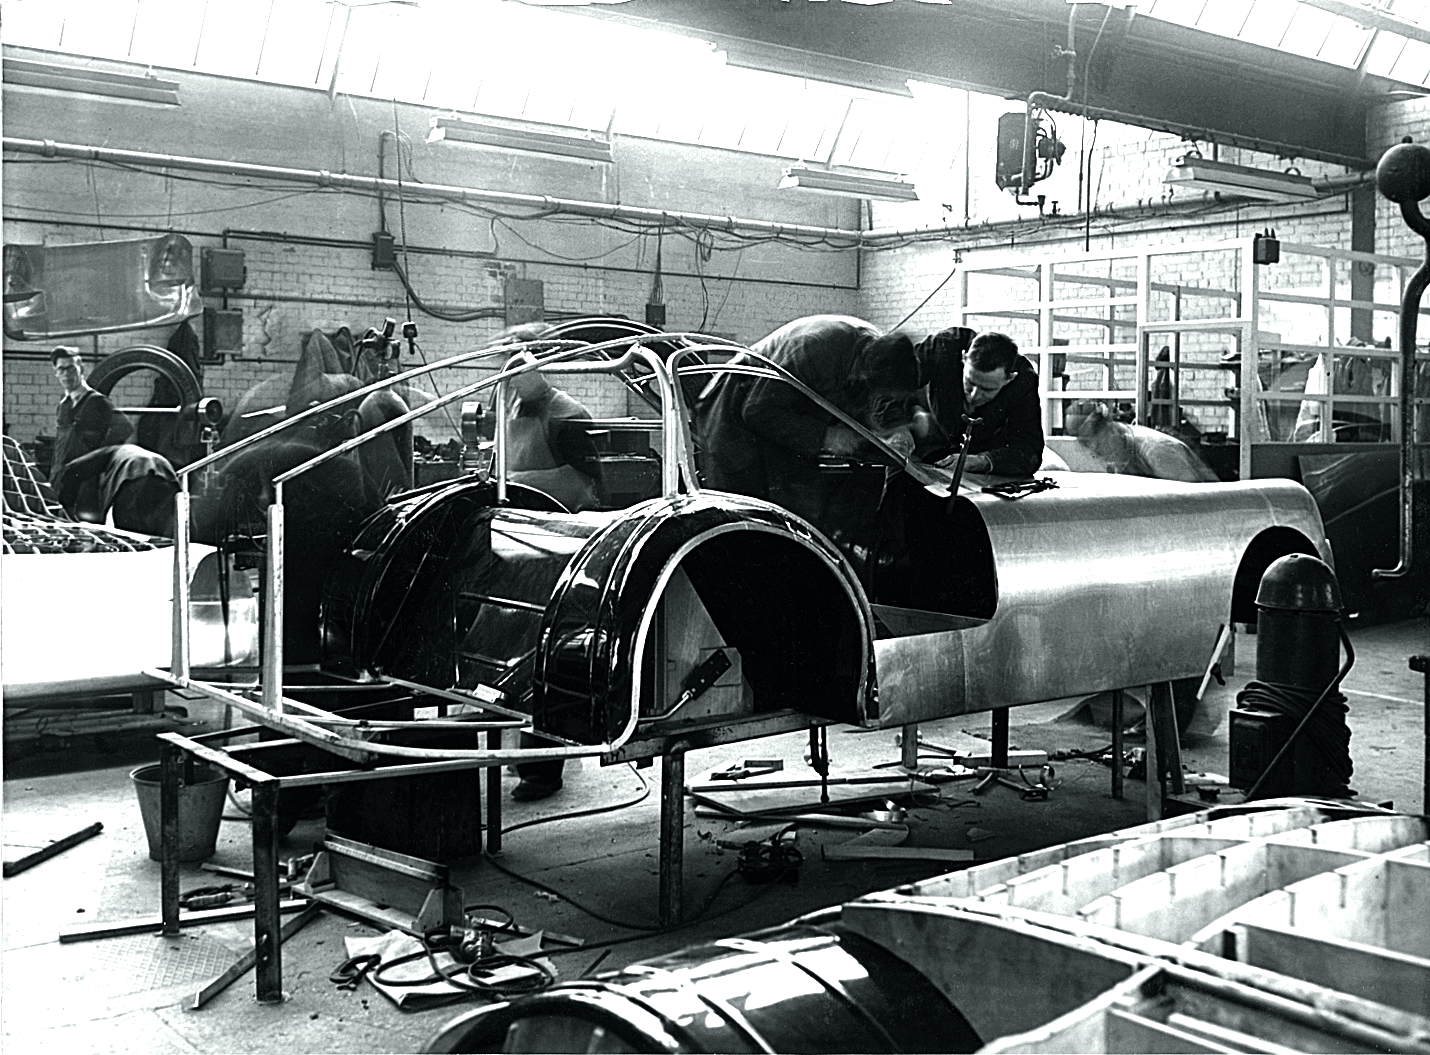
\includegraphics[height=5cm]{Images/OldCar.png}  
  \caption{Traditional hand-crafted car bodywork}
  \label{fig:OldCar}
\end{subfigure}
\begin{subfigure}[t]{.45\textwidth}
  \centering
  % include fourth image
  \includegraphics[height=5cm]{Images/Buck.jpg}  
  \caption{Modern-day hobbyist restoring a traditional buck}
  \label{fig:NewBuck}
\end{subfigure}\\[1ex]
%
\begin{subfigure}{.9\textwidth}
  \centering
  % include first image
  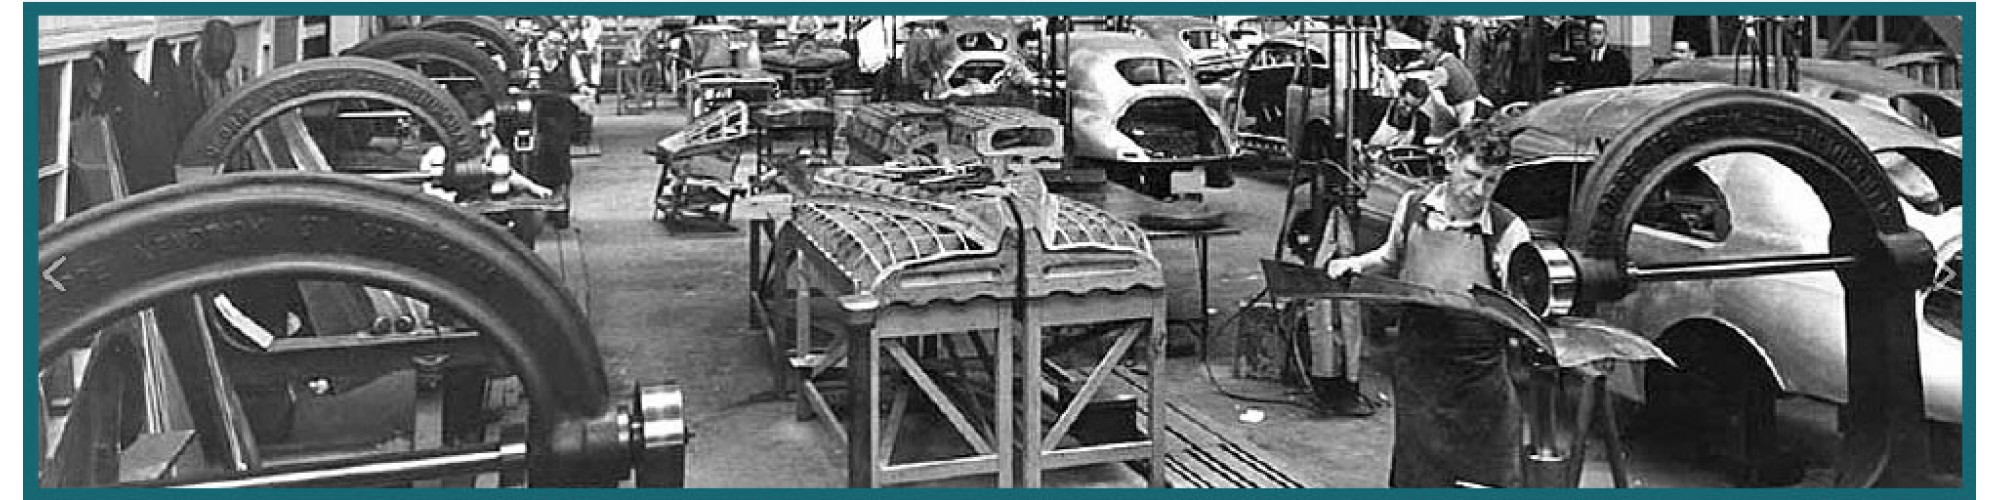
\includegraphics[width=\linewidth]{Images/OldFactory.png}  
  \caption{Panel beating factory}
  \label{fig:OldFactory}
\end{subfigure}
%
\caption{Traditional Metalsmithing. Images from Bristol Cars and Sam Frost Photos}
\label{fig:Background}
\end{figure}

The smith typically forms non-load-bearing panels for the automotive, aerospace and architectural sectors. Part geometries can be complex and include double curvature, for example the wheel fender body work shown in Figure \ref{fig:OldCar}. Becoming fully competent in the art of panel forming takes around 10 years of training \citep{Goodwin2020BehindBeaters}. The acquired skill set also equips smiths with the ability to repair damaged panels, with substantial implications for the servicing of a large range of products. However, the manual and laborious nature of this process results in a time-consuming and inefficient means of production by today's standards.

Unlike industrialised metal forming, there is no rigorous classification of processes/techniques used by the panel beater. This is further complicated by the colloquial language used to describe techniques and the ad hoc nature of some processes. Processes can be characterised as being fully worker controlled and actuated, often through manually handling both the sheet and tooling.

\begin{figure}[h]
    \centering
    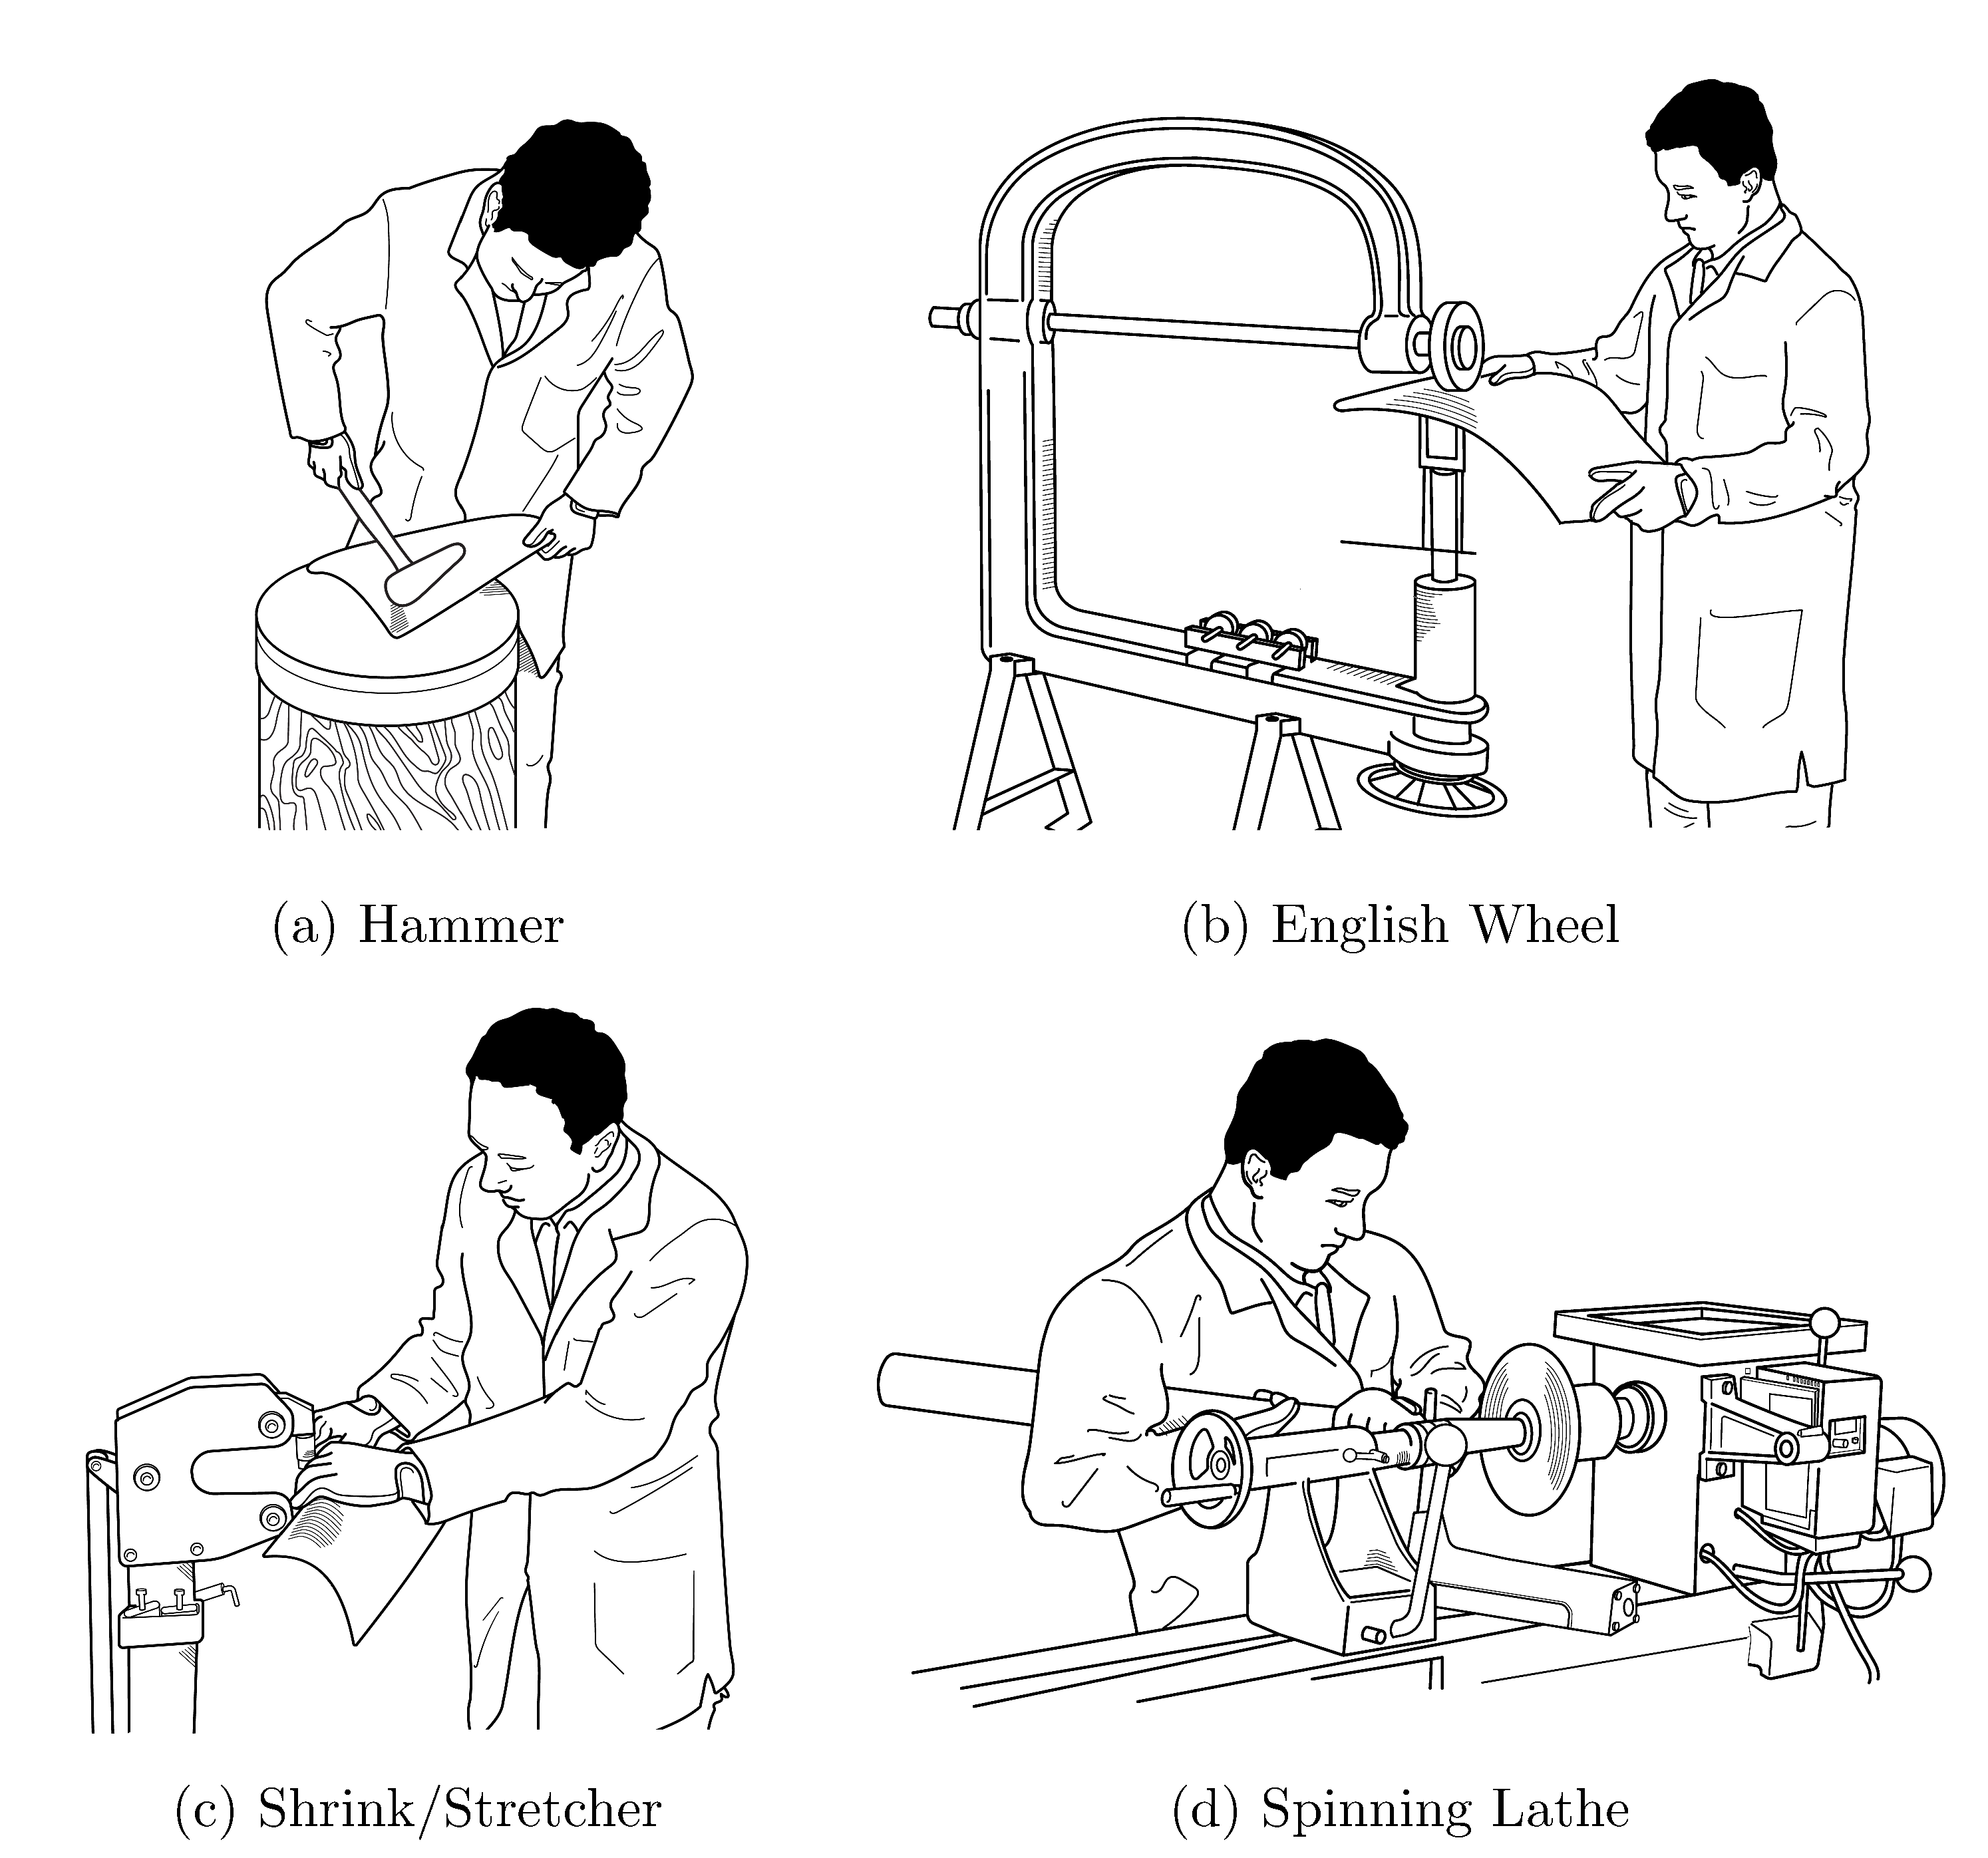
\includegraphics[width=0.8\linewidth]{Diagrams/Drawings.pdf}
    \caption{Tools used by the metal smith}
    \label{fig:Drawings}
\end{figure}

Four common tools are found in most workshops --- the hammer, the English wheel, the Kraftformer (or shrink/stretcher) and the spinning lathe --- all shown in Figure \ref{fig:Drawings}. These tools are used in many techniques to deform material, with each technique having a unique mechanism of deformation and forming capability. As a consequence of these individually limited forming capabilities, often a combination of different techniques are used in sequence to form parts. Correct selection of both tool and technique is crucial to successful part production, though different techniques can be used to complete the same job with selection of technique to the discretion and experience of the worker. A wooden or wire buck, as shown in Figure \ref{fig:NewBuck}, is often used to check the sizing of panels throughout forming.

Pre-dating the era of increased automation and high-volume production, sheet parts were often formed by these skilled smith in large factories --- see Figure \ref{fig:OldFactory}. These techniques have since been replaced with faster, more rigid processes to cope with demand. Alongside reduced flexibility, one of the unintended consequences of this change was the loss of the underlying expertise in the manipulation of sheet metal geometry.  Despite this decline in the number of skilled, professional smiths, the art of metal smithing is kept alive through a small community of enthusiasts and small number of job shops. 

\subsection{Tools and Techniques} \label{sec:ManualTech}
\subsubsection{Hammers} \label{sec:ManualHammer}

Hammers are perhaps the most crude tools used by the smith, but hammering is by no means the least complex technique. A typical posture for a metal smith hammering a sheet is shown in Figure \ref{fig:Drawings}(a), with both the hammer and sheet grasped by the worker and the sheet laid to rest on an anvil at waist height. Deformation occurs by repeatedly striking the sheet with the handheld tool against the supporting anvil, with the wrist of the worker providing some biomechanical stiffness \citep{Phan2020EstimatingTask}. The desired profile is incrementally formed by working across the face of the sheet.

The selection of both hammer and anvil is dependent on the technique used to form material and there is no definitive list of hammer sizes/shapes. Often hammers are personalised to both the workman and the job \citep{Barr2013ProfessionalFabrication}. Similarly, different anvils such as wooden dollies, cast anvils or sandbags are used for different jobs. Four main techniques can be used to shape the sheet using a hammer: folding, hollowing, raising and planishing as shown in Figure \ref{fig:hammertech}. 

\begin{figure}[h]
    \centering
    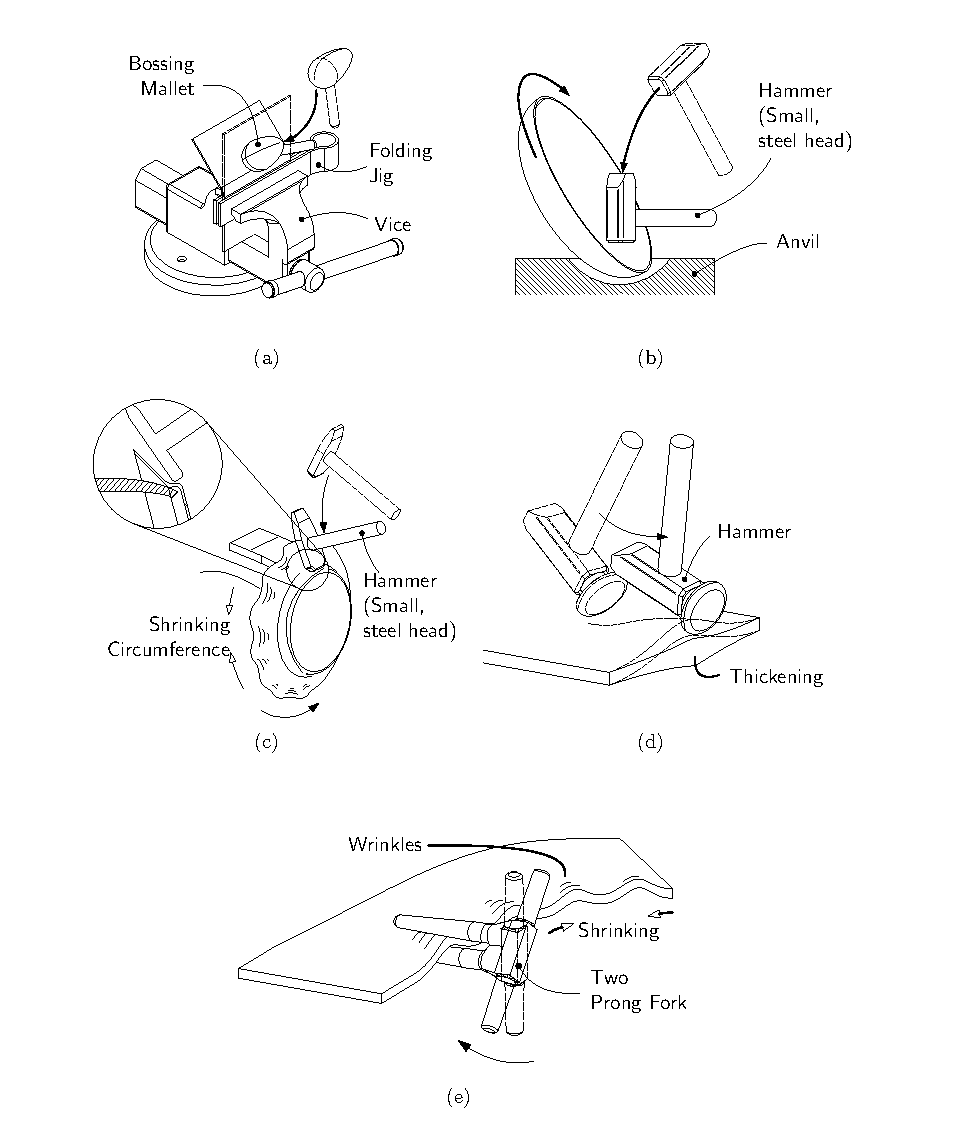
\includegraphics[width=0.75\textwidth]{Images/HammeringTechDrawing.pdf}
    \caption{Techniques using a hammer, adapted from \citep{Timings2008SheetMetalwork}}
    \label{fig:hammertech}
\end{figure}

Folding is perhaps the least complex hammering process where material is bent around the edge of an anvil, vice or holding jig --- see Figure \ref{fig:hammertech}(a). As this is a bending operation and no significant stretching occurs, curvature is only developed in one direction. For thinner sheets, this deformation can sometimes be carried out by simply bending the sheet by hand, or by pushing it around an anvil. However, using the momentum of a moving hammer both amplifies and concentrates the energy used to deform the material. 

Hollowing (sometimes called sinking) is used to form smaller compound curvatures or dishes, as shown in Figure \ref{fig:hammertech}(b). The workpiece is held at an angle above a compliant sandbag or above a wooden anvil with a crevice. The material is then struck with a large head hammer, sinking the material into the crevice/bag. The through-thickness compression causes thinning at the impact zone and spreads material outwards \citep{Music2012TheTools}. When forming a dish or a concave shape, following each blow, the workpiece is rotated and the process is repeated with each blow slightly overlapping the previous. In forming a bowl, the impact locations begin at the outer edge and spiral toward the centre as the sheet is rotated.

Raising is a more complex hammering process that allows larger curvatures to be formed \citep{Livesey2019TheBodies}. To start, the workpiece is given a slight curvature by hollowing and placed onto the edge of an anvil. Using a smaller, heavier head hammer, material is struck just beyond the edge of the anvil, forcing it down and around the anvil, shrinking and reducing the circumference of the workpiece, as illustrated in Figure \ref{fig:hammertech}(c). The sheet is rotated and the process repeats, spiralling from the centre, to the outer edge. Wrinkles that arise from reducing the circumference are worked out by skilfully thickening the material by striking the base of the wrinkle, bringing together each side of the wrinkle --- see Figure \ref{fig:hammertech}(d).  Raising can also be carried out by tucking the edges of the workpiece, reducing the circumference by folding material at the edge over itself into a wrinkle using a two prong fork --- shown in Figure \ref{fig:hammertech}(e). 

Smaller, flat-head hammers are used to planish imperfections from the surface of a worked sheet. By carefully striking high spots on the sheet, the material thins and spreads outwards, leaving an improved surface finish. A hard anvil is normally used during this process. There are several variations of planishing hammers called ``spoons'' and ``slappers'' which are suited to the task of planishing \citep{Barr2013ProfessionalFabrication}. 
Repair work can be carried out without having to remove panels and place them on an anvil by using small, hand-held dollies or a ``bulls-eye pick'' which mounts a hammer and anvil on a hinged C-shaped jaw-frame. This can be actuated at the base of the frame allowing the worker to access and planish difficult to access areas.


\subsubsection{Kraftformer} \label{sec:ManualKraftformer}

The Kraftformer machine is the commercial name for the more widely known `shrink/stretch machine' --- shown in Figure \ref{fig:Drawings}(c) --- made by Eckold \citep{Unknown2020ECKOLDBrochure}. A C-shaped frame houses a reciprocating press that is actuated manually by a foot pedal or is mechanised in such a way that both the depth of stroke and the number of strokes per minute can be adjusted. Several different tools can be fitted to the end of the press of a Kraftformer, each translating the vertical motion of the press to deform the workpiece in a distinct manner. A schematic of eight different tools specifically used to form sheet metal is shown in Figure \ref{fig:Kraftformer}, although other tools are available \citep{Unknown2020ECKOLDBrochure}. Traditional shrink/stretch machines, like the one shown in Figure \ref{fig:Drawings}(c) come with fewer tools.

\begin{figure}[h]
    \centering
    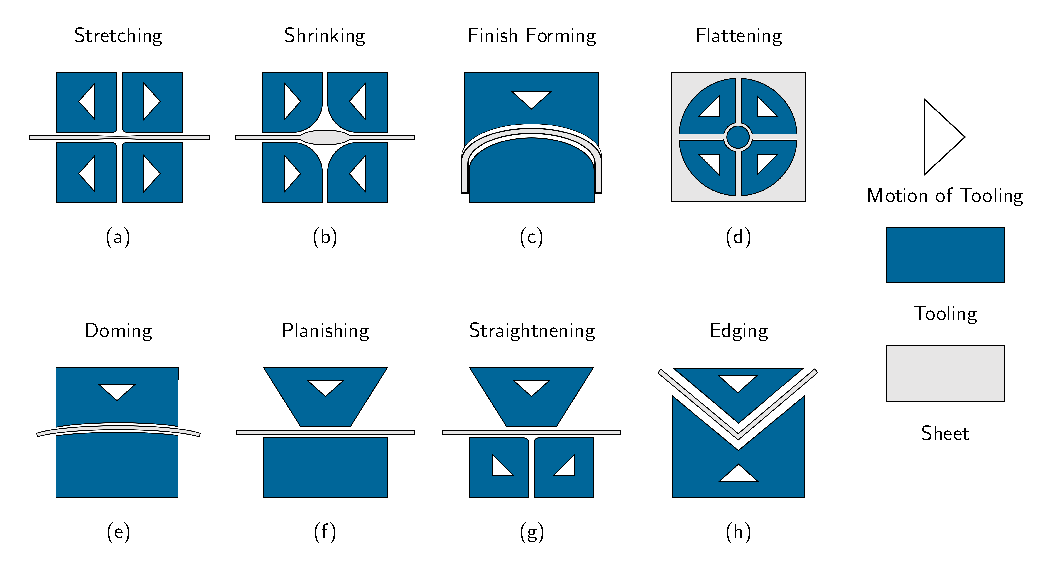
\includegraphics[width=0.7\linewidth]{Images/KraftformingTools4x2S.pdf}
    %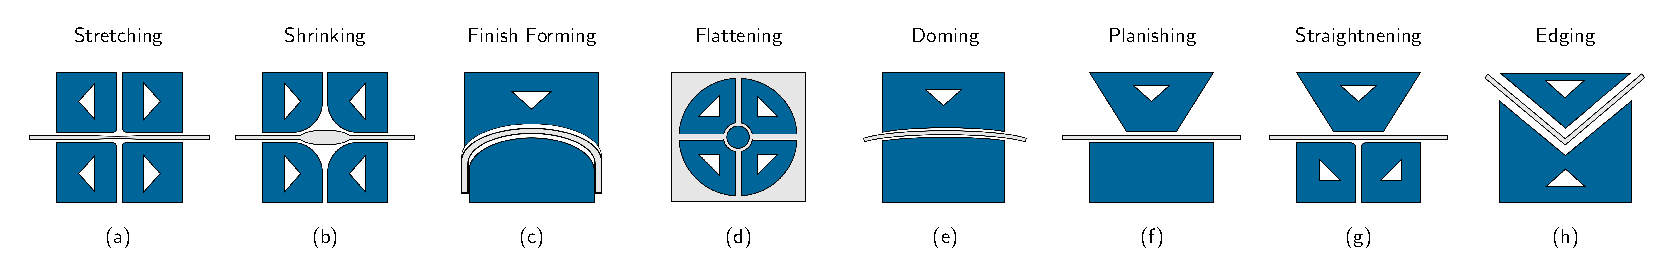
\includegraphics[width=0.95\linewidth]{Images/KraftformerTools8x1.pdf}
    \caption{Kraftformer Tools, adapted from \citep{Unknown2020ECKOLDBrochure}}
    \label{fig:Kraftformer}
\end{figure}

The shrinking, stretching and doming tools are often used to form curved sheets. The doming tool deforms material similarly to the hollowing technique used in hammering, although the stretching and shrinking tools are more elaborate. When using these tools, each stroke brings together the upper and lower tools toward the sheet until it is clamped. The remaining vertical motion of the stroke is translated into horizontal movement via a linkage, with the tools moving outward or inward, stretching or shrinking the sheet respectively. Different designs of shrink/stretch tooling have been developed and patented \citep{Joyner1943SheetMachine,Rusch2011ShrinkerMachine,Eckold1950ToolElements,EckoldWalter1954ApparatusProfiles}.

When driving (the term for operating a Kraftformer), the smith stands beside the machine, with both hands holding the sheet and resting it between the jaws of the press. As the press reciprocates, the sheet is manoeuvred through the jaws by the worker and is incrementally formed. The repeated deformations incrementally deform the sheet and gradually a shape is generated. A combination of tooling may be used during processing, especially when both concave and convex curvatures are required. The maximum pressure that can be exerted on the sheet varies with different models of Kraftformer and scales with the size of the machine \citep{Unknown2020ECKOLDBrochure}.

\subsubsection{English Wheel} \label{sec:ManualEW}

The English wheel, sometimes called a wheeling machine, is primarily used to form or planish sheets of compound curvature. A typical wheel consists of a C-shaped frame with two anvil rollers mounted between the jaws of the frame. Frames can be fabricated from steel box section or cast as one piece. Cast frames are more desirable as they are more inflexible, resulting in a more consistent surface finish. The upper anvil roller has a flat profile, whereas the lower anvil is crowned to accommodate curvature in the sheet in the transverse to rolling direction. This lower tool can be quickly changed to another tool with lesser, greater or no crown and the gap between the rollers can be finely adjusted to change the pressure of the tool on the sheet. 

Wheeling (the process of using an English wheel) is renowned as a complex task capable of forming intricate, smooth curves, whilst leaving an aesthetically pleasing finish and good surface quality \citep{Longyard2014LearningWheel}. Similar to driving, the worker stands beside the machine with both hands on the sheet placing it between the rollers. By raising the lower anvil roller, the sheet is pinched between the two rollers. The worker then manoeuvres the sheet back and forth between the two anvil rollers, gradually tracking across the face of the sheet in a `zig-zag' pattern as shown in Figure \ref{fig:WheelingTech}(b). To ensure a quality finish, the tracking angle between each pass should be small enough that back and forth strokes should slightly overlap and the pressure on the sheet should be limited.  

\begin{figure}[h]
    \centering
    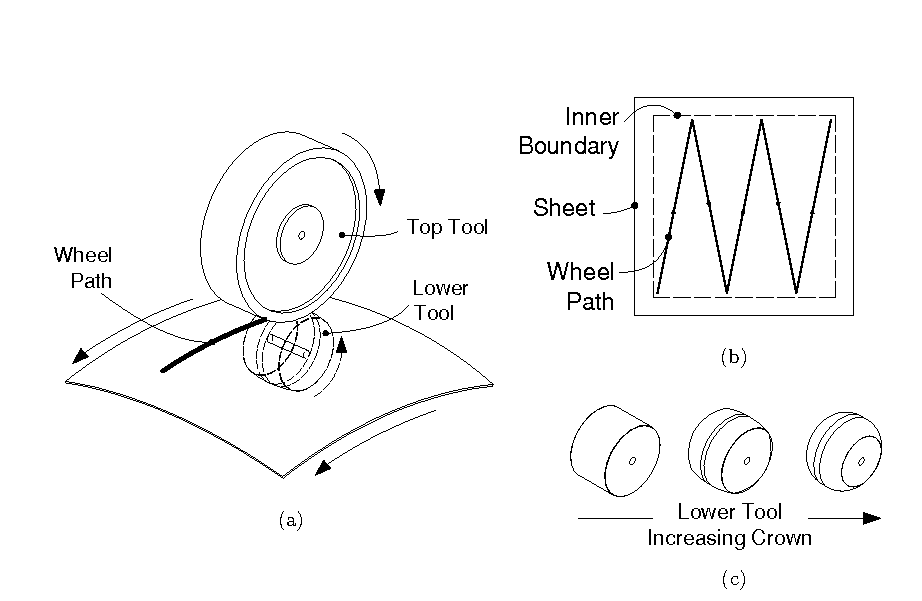
\includegraphics[width=0.8\linewidth]{Images/WheelingTechDrawing.pdf}
    \caption{Wheeling Techniques and Tools}
    \label{fig:WheelingTech}
\end{figure}


The deformation of the sheet between the tools is a combination of stretching and bending with the anvils thinning and displacing material outward away from the tools \citep{Bowen2021NumericalProcess}.  This deformation mechanism can be used to form regions of double curvature from an initially flat state by a technique known as stretching. This technique involves wheeling across the face of the region, whilst leaving an outer boundary unwheeled. The thinned, stretched material on the inside of this boundary is constrained by the unwheeled outer boundary which causes it to rise out of plane, resulting in double curvature. Alongside this, the English Wheel is often used to planish wrinkles from previous operations, such as hammering.

\subsubsection{Spinning} \label{sec:ManualSpinning}
Hand spinning is a process in which the smith forms axisymmetric parts from flat sheets using a lathe and a manually held tool. A mandrel (also known as `chuck’ or `former’) shaped to a desired profile is mounted to the headstock of the lathe with the sheet mounted in-line and held in place with a follower, clamped by the tailstock. When spinning, the smith stands beside the machine and controls both the rotational velocity of the spindle and the trajectory of the forming tool. With both the sheet, mandrel and follower rotating, the smith applies pressure to the workpiece using the forming tool, which travels radially from near the centre of the blank to its outer perimeter and back in rapid strokes. This causes the workpiece to progressively deform and eventually take the shape of the mandrel.

There is no standardised set of tooling used in spinning. Instead, smiths often create their own tooling which is tailored to the individual user and sometimes to a particular job. These tools are typically long metal sticks with a suitable geometry at one end and a wooden handle at the other. A tee-rest with a movable fulcrum pin is sometimes used to allow the smith to apply higher forces whilst maintaining precise control over the motion of the tool. A wooden backstick is also commonly used during the forming stage to prevent wrinkling of the workpiece, which is especially likely when the blank is slender \citep{Jawale2019AnSpinning}. Lubrication is routinely used to reduce heating, increase formability and avoid scratching the workpiece.

As the overall perimeter of the sheet from the initial to the final shape reduces, the process is prone to circumferential wrinkling. This can be balanced by allowing the workpiece to elongate radially, but excessive elongation leads to tearing. Thus, the craft of spinning consists in progressively forming the blank while avoiding both wrinkling and excessive elongation and many years of practice are required to successfully form a variety of geometries and materials without failure \citep{Holtzappfel1852TurningManipulation,Tuells1912MetalUsed}. The shape of the workpiece, its resistance to deformation and the sounds it makes are all cues for the smith to understand how to successfully form it.

Different techniques are used to successfully spin desired parts, whilst avoiding wrinkling and tearing failure mechanisms. The sheet can be initially formed against the mandrel using one of two techniques. Deeper parts with cup-like geometries must be spun in multiple passes. A conventional multi-pass forming technique uses both forward and backward passes to gradually form the part. The early strokes are used to lay down material onto the central chuck or mandrel so as to increase process stability. Thereafter, forward and reverse strokes are used and most deformation concentrates around the tool, which gradually traverses the entire part. The speed of traverse, and degree of deformation per pass are both carefully controlled by the Smith so they remain within safe upper and lower limits. As a result, the intermediate forms tend to take a concave shape, as shown in Figure \ref{fig:SpinningTechDrawing}, since the edge of the part is most vulnerable to wrinkling and must be deformed less. 

Shallower parts with a conical shape can be formed in a single pass, in a technique known as shear spinning. In this, a tee rest and elongated tools are used for a greater mechanical advantage allowing the smith to exhort the greater force needed to complete forming in a single pass. The stroke is usually terminated before the edge of the workpiece is reached, and so the process usually results in part of unchanged outer diameter. 

With the part formed against the profile of the chuck, a finishing technique is used to remove any spinning lines.  This involves using a flat sided tool to run over the part to smooth out any imperfections.  Some other specialist techniques are described in \citep{Wiley2004TheHand-spinning}.  These include techniques to form re-entrant shapes, which require a split mandrel, and even fully folded back flanges, which require the use of spinning pliers. The latter a highly skilled and dangerous operation since the tool must access the spinning cavity. Furthermore the techniques of trimming and annealing are used to correct for anisotropy and out of roundness, and restore formability of difficult to work materials respectively.  

\begin{figure}[tbh!]
    \centering
    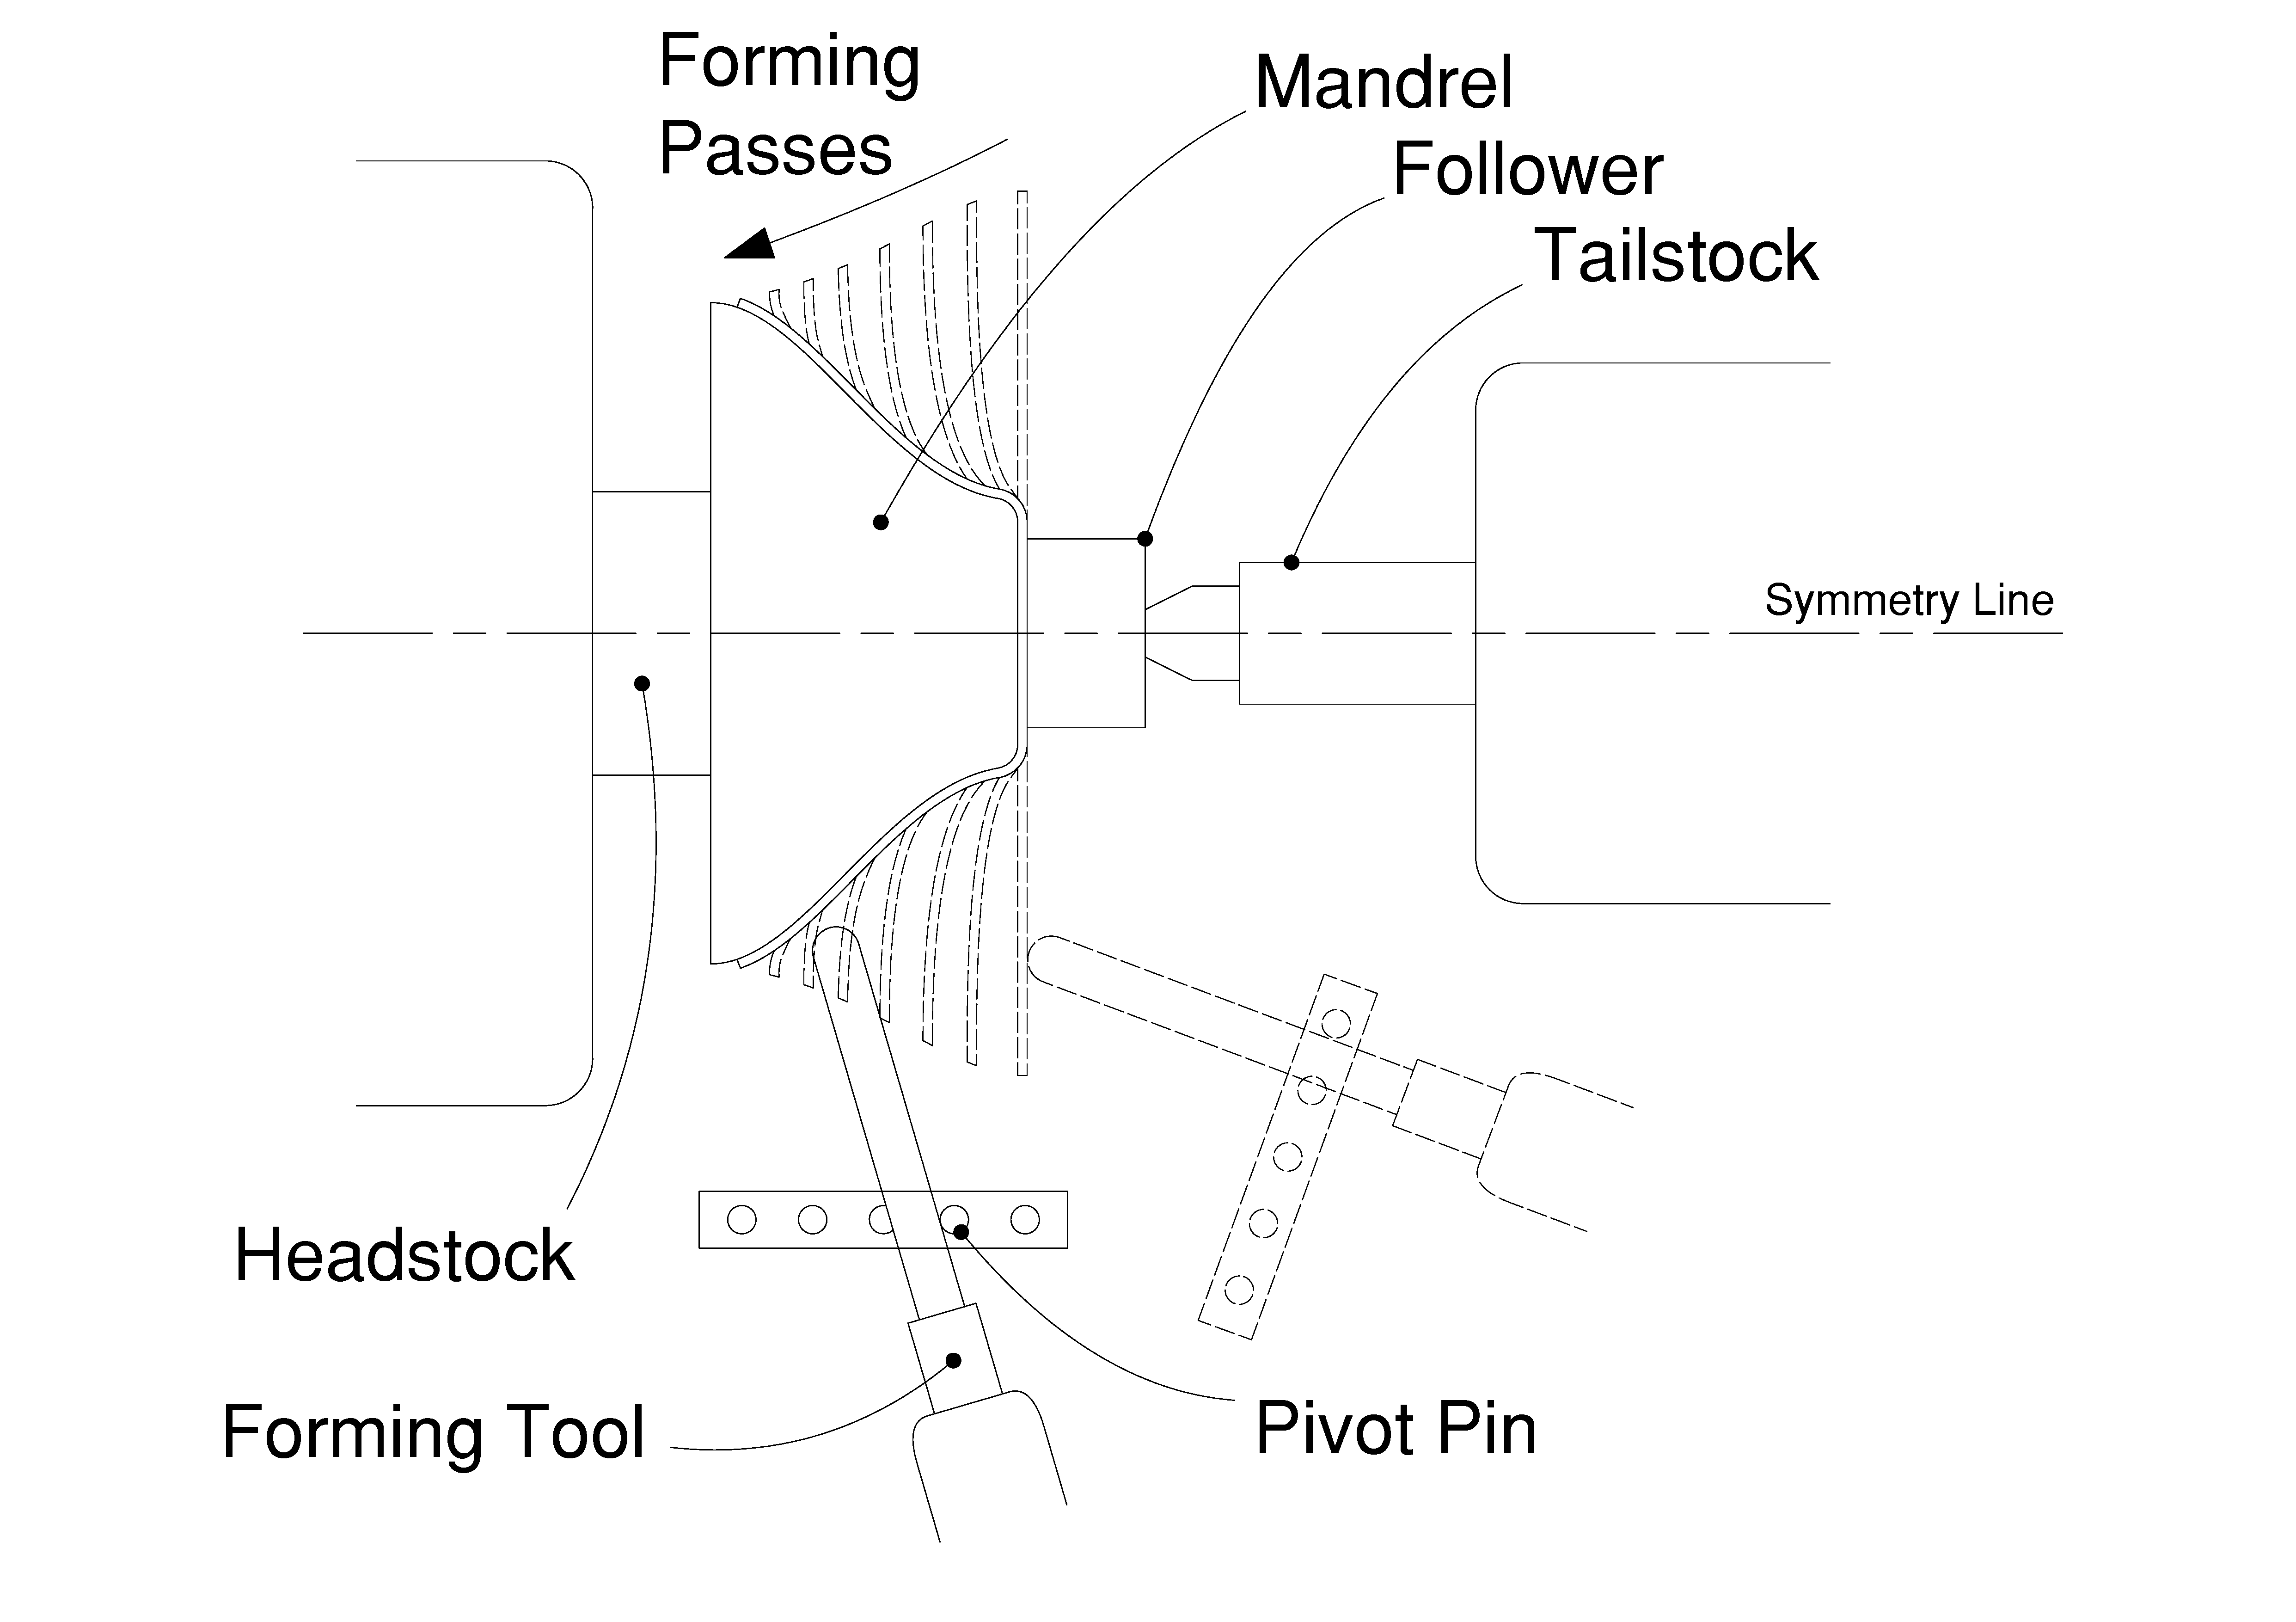
\includegraphics[width=0.6\linewidth]{Images/Spinning.pdf}
    \caption{Hand spinning}
    \label{fig:SpinningTechDrawing}
\end{figure}

%%%%%%%%%%%%%%%%%%%%%%%%%%%%%%%%%%%%%%%%%%%5

\subsection{The smith's tacit knowledge} \label{sec:tacitknowledge}

A thorough understanding of the fundamental techniques used to form a sheet does not fully guarantee successful part production on its own. As the smith works towards a target shape, their techniques will continually be adjusted based on the sensory feedback. Indeed, successful crafting is not just the application of movement and force to a workpiece, but requires qualities of care, judgement and dexterity \citep{Pye2008TheWorkmanship}, where dexterity is not just coordinated bodily movement, but the craftsman's response to the ever-changing conditions of the workpiece \citep{Ingold2001BeyondSkill}. In line with reviewing the physical techniques used by the smith, it is also valuable to consider their cognitive process when working.

We define the smith’s cognitive process as the forming strategy. This encompasses the many different decision-making elements taken by the smith when creating a desired part. This includes decisions made prior to forming, such as the selection of technique or combination of techniques to be used and any pre-processing operations to the blank. During forming, decisive elements such as tool trajectory and machine settings are chosen alongside more subtle factors, such as the boundary conditions imposed by the smith as they grasp the sheet. Specifying the correct forming strategy is key to successful part production.  

Consider the smith using a hammer to hollow a dome from a flat sheet as part of fabricating a motorcycle fuel tank as described in \citep{Barr2013ProfessionalFabrication}. In this process, there are three main elements: the sheet that is to be deformed, the tool to carry out the deformation and the smith, who provides controlled actuation of both tool and workpiece. The smith is a source of both energy (in the form of manual actuation) and information (in the form of a decisive strategy), the combination of which gives controlled movement of both the tool and sheet in a trajectory described as a manufacturing strategy. Through the tool, energy is transferred into the workpiece causing deformation, though in some processes such as spinning or driving, the energy used to deform is partly sourced from the machine and is regulated by the worker. Energy is also used to manually manoeuvre the sheet. Throughout forming, the worker continuously receives feedback from everything they are interacting with: force from the tool and sheet as well as other sensory stimuli through the environment (visual and audio feedback). 

\begin{figure}[h]
  \centering
  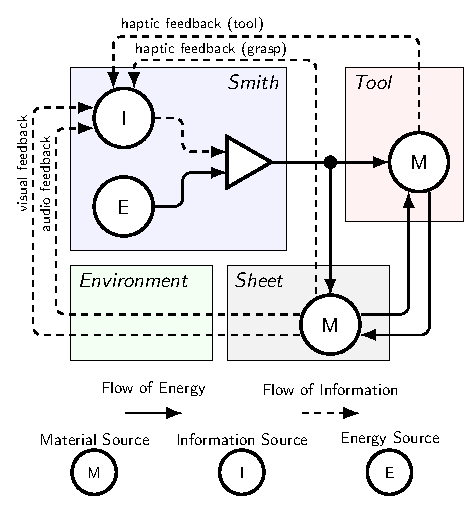
\includegraphics[width=0.5\linewidth]{Diagrams/DAP4.pdf}  
  \caption{Design activity pattern}
  \label{fig:DAP}
\end{figure}

Using this information, a design activity pattern for manual sheet forming is mapped in Figure \ref{fig:DAP}. As well as showing the exchange of energy between smith, sheet and tool which causes deformation, this demonstrates the diverse range of feedback data received by the smith when working. Similar analysis on other skilled manual manufacturing processes such as wood cutting \citep{Roth1981FoundationDesign}, welding \citep{Zhang2012ModelingPrinciples} and generally for Human-Physical systems \cite{Zhou2018TowardManufacturing} also demonstrate the presence of these feedback cues. Understanding how this feedback information is processed to determine how manufacturing strategy is both generated and adapted is a widely covered topic and beyond the scope of this paper. Broadly, in information processing models such as those by \cite{Wickens2015EngineeringPerformance} and \cite{Endsley1995TowardSystems}, decisions are informed as a result of the perception of external stimuli (the feedback data), attention resources (tiredness, surrounding environment etc.) and both long term and working memory (past experiences). This is emphasised by Wiley: ``\textit{Experienced spinners are keenly aware of how metal will react under certain situations and have a built-in sense of impending danger milliseconds before disaster strikes, programmed from years of near misses}'' \citep{Wiley2004TheHand-spinning}.  

As parts produced by the smith are often made from constituent complex geometries, forming an overall shape often requires multiple operations, utilising different techniques. In the earlier motorcycle fuel tank example, hollowing is just the first stage of production with raising and wheeling techniques subsequently used to form the shape, alongside other auxiliary processes such as cutting, welding and finishing operations \citep{Barr2013ProfessionalFabrication}. Selection of tooling/technique is part of the smith's tacit logic and is further complicated by process selection variability within manual processing. This is demonstrated in Figure \ref{fig:ShapeDevBow}, which outlines various ways in which the smith might form a deep bowl using different tools and techniques. The choice of technique will be based on the smith’s individual skills, past experiences and availability of tools. 

\begin{figure}[h]
    \centering
    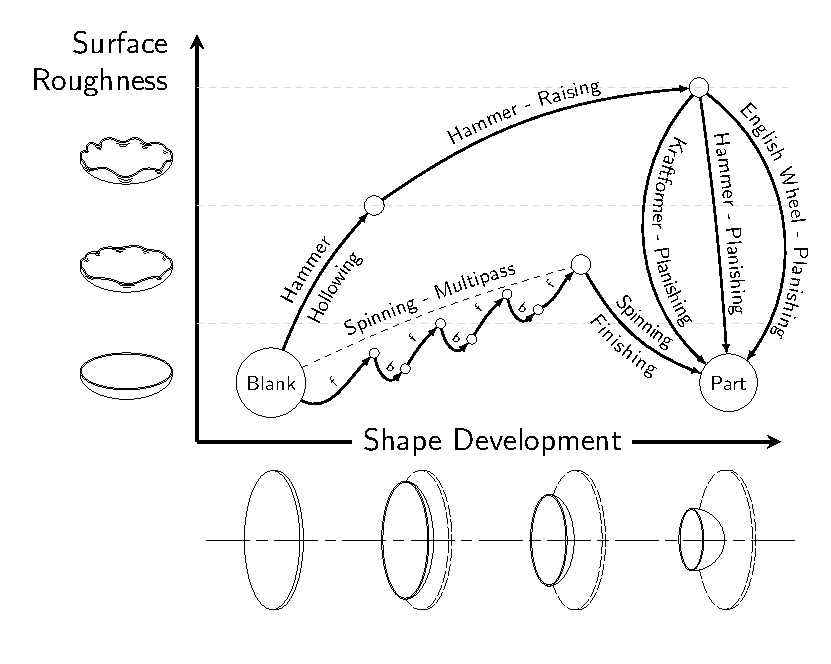
\includegraphics[width=0.6\textwidth]{Images/Bowlv2.pdf}
    \caption{Distinct manufacturing strategies using multiple techniques to form a deep bowl}
    \label{fig:ShapeDevBow}
\end{figure}

%Crafting, and its alignment with both art and design is a widely discussed topic \citep{risatti2009theory}. A useful focal point on craft is one by Roman author Vitruvius in \textit{De Architectura}, where the craftsmanship of the experienced architect is described in two elements, \textit{fabrica} and \textit{ratiocinatio} \citep{vitruvius_1999}.\textit{Ratiocinatio} is the underlying thinking and purpose of the object, rather than the concrete thing whereas \textit{Fabrica} is the craftsmanship that grows out of fabricating a material work when working toward a proposed design \citep{Poerschke2016}. It is held that the nature of craft lies in the perfect realization of a form before the work begins. We focus our attention on the \textit{fabrica} element of crafting; the process of creating a specified desired form from an initial workpiece and the inherent ability that enables the craftsman to carry this out successfully.



\newpage
\section{Mechanised Metal Smithing} \label{sec:Mechanised}

Some of the versatile, manual techniques developed by the metal smith have been used as starting points for the development of new flexible automated processes. Here we review some new processes that are derived from or analogous to traditional processes, focusing on the hardware and control systems used to automate production.


\subsection{Processes} \label{sec:MechanisedProcess}
\subsubsection{Automated Hammering} \label{sec:MechHammer}
Identifying processes that can be considered as automated hammering is not straightforward as the definition can be associated with a number of different incremental forming processes \citep{Emmens2010TheHistory}. Larger mechanised hammers are used in processing bulk material \citep{Lange1986HandbookForming} and Kraftformers can be fitted with doming tools for mechanised hollowing --- see Figure \ref{fig:Kraftformer}(e).

Novel processes have been developed that take inspiration from different manual hammering techniques. The technique of raising for example --- see Figure \ref{fig:hammertech}(c) --- has inspired the development of a novel spinning process which allows deeper bowls to be formed compared to traditional spinning \citep{Russo2020RaisingSpinning}. In this process, the deformation mechanism used during the manual technique is replicated, substituting the hammer and anvil with working and support rollers respectively. The folding-shearing process is another example of a raising-inspired process which closely replicates the smith's technique \citep{Allwood2019Folding-shearing:Change}. Although they make no reference to the traditional smith, Yoon and Yang developed a process where a hemispherical tool is used to punch sheets into a crevice, akin to hollowing \citep{Yoon2001InvestigationMetal}. 

Researchers at Loughborough University's intelligent automation centre used an industrial robot arm to manoeuvre a sheet through a Kraftformer machine with a doming tool fitted. Though a Kraftformer is used, throughout the development of the process, the designer refers to the hammer hollowing technique as inspiration for the process \citep{Ilangovan2016FixturelessForming}. A novel control method is developed to regulate the process --- Mechatroforming. This method uses data collected from a skilled smith including impact force, trajectory and impact angle as well as data collected from finite element simulations to specify both the impact location and magnitude of force required to shape a desired part \citep{Ilangovan2016AnForming}. The system also uses feedback sensors in regulating the process, scanning the geometry of the sheet at regular intervals, alongside continually measuring the impact force during forming.

A number of processes utilise a hammering technique to deform material, though the sheet is clamped at the outer edge. Tanaka develops such a process, using a \textit{yani-dai} anvil --- a plastic hammering support base with pine resin used in Japanese traditional artistic forging work. Initially, forming strategies are generated by specifying impact locations which map out the desired part shape using a selected pattern (spiralling inward/outward or contouring) for simple shapes \citep{Tanaka2005DevelopmentWorking} and for NURBS surfaces created in a CAD environment \citep{Tanaka2012DevelopmentSystem}. The system is later developed to account for the developing deformed surface, using a parametric curve interpolation  \citep{Asakawa2010DevelopmentProcess} and to also adjust the impact angle on the face of the sheet as the part is formed \citep{Takasugi2012DevelopmentShape}. A similar process is developed by Mori who uses a genetic algorithm to determine manufacturing strategy. The algorithm works by optimising the manufacturing strategy for a desired geometry using an empirical model to simulate deformed geometry (specifically local curvature) for a given strategy. Data was obtained through FE simulation and physical experiments \citep{Mori1996DeterminationAlgorithm}. 

Some other processes that constrain the edge of the sheet use sensors as an integrated part of the manufacturing strategy. For example, a two-stage process developed by Mori firstly hollows the part into the desired shape, having selected a strategy from a database of strategies captured experimentally through systematic variation of impact positions and depths. Then, a camera is used to identify imperfections in the workpiece and the sheet reworked in these areas (akin to hollowing and planishing) \citep{Mori1998IncrementalDatabase}. The previously mentioned system developed by \cite{Tanaka2008FormingMeasurement} is also designed to measure errors both after forming to subsequently modify strategy and during forming to provide online geometry feedback, resulting  in reduced deviations with desired part shape \citep{Tanaka2014DevelopmentHammering}. A machine is under development at the Fraunhofer Institute where, although manufacturing strategy is manually selected by the operator, a flexible holding system is used which adapts to the shape of part as it is formed \citep{Sharon2014FraunhoferReport}.

Variations of the well-established incremental sheet forming (ISF) process were created such that the sheet is repeatedly impacted (hammered) into position. These are sometimes referred to as incremental sheet punching (ISP) processes. Some example configurations of these processes include using a CNC or traditional mill to incrementally punch material with a static forming tool \citep{Wang2017IncrementalPath,Zhu2019ToolForming}, or use a bespoke reciprocating forming tool to hammer material, mounted either as an end effector to a 6-axis robot arm \citep{Schafer2005IncrementalRobots, Puzik2008IncrementalApplication, Luo2010AResults}, or to a CNC mill \citep{Asgari2017DesignDamper}. The manufacturing strategy is defined using analytically derived methods, such as the ones described in \cite{Schafer2005IncrementalRobots,Wang2017IncrementalPath,Zhu2019ToolForming,Luo2010ASimulation}. However, in these processes, the sheet is clamped at the edge, a supporting anvil is not used and there is no reference to the traditional smith and their techniques.
 

\subsubsection{Automated Driving (Kraftformer)} \label{sec:MechKraftformer}
In all known cases to the authors, attempts to automate the process of driving stem exclusively at the Technical University of Munich. Developments focus on the generation of manufacturing strategy – specifically the impact locations on the sheet, using a traditional Kraftformer tool with stretching tools installed. For processes where the physical movements are automated, the sheet is manipulated using a 6 axis industrial robot arm.

The challenges associated with generating an automated manufacturing strategy using analytical methods were identified early in the development process \citep{Golle2007DrivingProducts}. Instead, `knowledge based' and `cognitive' approaches were suggested. Knowledge-based systems derive new strategies from strategies captured from physically formed sheets whereas `cognitive' strategies used data collected from sensors to adapt the strategy when forming online in real time --- similar to the traditional smith. An early example of this cognitive approach is the development of a system to assist manual driving, which allows the worker to check the geometry of the part they are forming in real time, without having to remove the sheet from the machine, by scanning in the geometry and overlaying this with the desired geometry on a head up display \citep{Scherer2010DrivingProducts}.

There are many ways in which the knowledge-based approach has be implemented. Initially, \cite{Hoffman2009AnHandling} captured the manufacturing strategy used to manually form a sheet (impact forces and positions on the sheet) then translated this data to allow for a industrial robot to handle the sheet and repeat the process, thus replicating the part. % An See [10] in `Automated driving by standardizing and scaling the manufacturing strategy'
Later, efforts were made to eliminate the need to explicitly capture a manufacturing strategy required to create a desired geometry. This was done by capturing and scaling the manufacturing strategy (the impact locations on the sheet) of a physically formed shape with a desired geometry \citep{Opritescu2012AutomatedStrategy}. Later, more sophisticated methods of scaling manufacturing strategy were used, utilising statistical methods to enhance the value of the data collected \citep{Opritescu2016VariationVariance,Hartmann2019Knowledge-basedPartitioning}.

Other methods have been used to specify manufacturing strategy and investigate the deformation mechanics. A novel, more computationally efficient approach using a purely geometric model to demonstrate the change of 3D-forms has been developed, where the respective forming parameters are identified through experiments \citep{Yang2011GeometricalProcess}. Model Predictive Control (MPC) has been used to define an optimal manufacturing strategy for shaping L-shaped channel sections, based on an analytically derived deformation model \citep{Yang2009AutomatisierungProgramming}. The process has also been simulated using the finite element method \citep{Hoffmann2005StudiesMetal}. However, the high computing time and lack of flexibility in the modelling process were deemed impracticable for developing manufacturing strategies \citep{Scherer2013MethodenBlechumformung}. 

Recently, neural networks have been used to specify manufacturing strategy. In one such example, L-shaped profiles were formed into shapes with curvature along only one dimension to reduce complexity \citep{Opritescu2015AutomatedApproach}. The network architecture was designed to input the desired geometry --- specifically the curvature along the surface along with material parameters and the resulting output specifies manufacturing strategy (sheet trajectory through the tools). The network was trained using toolpaths and geometries collected through experiments. This strategy was later developed towards more complex sheet geometries by significantly pre-processing the data before training the network \citep{Hartmann2019AnFree-forming}.

\subsubsection{Automated Wheeling} \label{sec:MechEW}
The English wheel has received little attention, with only two known attempts to automate the process identified by the authors. Both these processes use a traditional tool with the worker replaced by a 6 axis industrial robot arm and only one machine configuration is considered. 

US architectural company Zahner investigated the feasibility of the process for industrial applications. To form a desired compound curvature, the manufacturing strategy was specified using a rule-based system where patches of high Gaussian curvature on the surface of a desired shape were identified and a trajectory along the face of the sheet to be wheeled was constructed such that patches of greater curvature were wheeled more often. Though no detailed results are published, the researchers stated that doubly curved panels with curvature were successfully formed and were ``in good alignment with predictions'' \citep{Vazquez2017RoboticWheeling}. 

Having identified the complex nature of the wheeling process, Rossi and Nicholas used a neural network (NN) to generate a toolpath, citing the system's ability to capture complex behaviour that rule-based systems cannot capture \citep{Rossi2018ModellingWheel, Rossi2018Re/LearningSurfaces}. The network was trained using data collected from tracking the manufacturing strategy and final geometry of six physically wheeled sheets. This data was augmented by orienting and subdividing the panels to increase the amount of training data available for the NN. A Kinect device was used to scan the sheet during forming to continuously recalculate the position of the arm to correctly position the sheet between the anvils whilst accounting for the developing curvature of the sheet. The system architecture was constructed such that every new sheet that is fabricated is used to improve the neural network.

In both these automated processes a high tool pressure is exerted on the sheet. Alongside explicitly stating this, this is evident from the makings left on the sheet post forming and the high levels of deformation seen after just a few passes through the tools. Traditionally, low pressure is used to gradually form the sheet over many passes, leaving a smooth, unmarked finish. Studies have shown that higher tool pressure leads to the sheet bending rather than stretching \citep{Bowen2021NumericalProcess} which suggests that these automated processes do not make use of the stretching technique used by the traditional smith.


\subsubsection{Automated Spinning} \label{sec:MechSpinning}

The process of hand spinning, as described in Section \ref{sec:Manual}, has undergone progressive automation over the course of the second half of the 20$^{\text{th}}$ century. Initially, two major requirements drove innovation: the need to spin larger and thicker parts, which required higher power than a human could deliver, and the need to spin larger quantities of parts faster \citep{Wong2003AProcesses}. More recently, flexible metal spinning processes have been at the forefront of development \citep{TheUseLessGroupFlexibleSpinning}.

%This led to the requirement to automate  automation of , for example, to the use of the compound lever to exploit mechanical advantage and spin thicker workpieces; then, hydraulic lathes were introduced to apply even higher force. 

Initially, production rates were improved by implementing template copying control and eventually computer numerical control (CNC) into spinning machines in the 1970s. These processes had automated the physical actions of the hand spinning process, toolpath with manufacturing strategy directly programmed by the worker. Wong et al report that the need for experienced spinning operators with programming skills made CNC machines problematic \citep{Wong2003AProcesses}. Thus, in the 1980s, teach-in/playback systems known as PNC (programmable numerical control) were introduced \citep{Lloyd1986AnProspective}. In these systems, an experienced smith forms a part while their actions are recorded by a computer. This is then played back automatically to make the same parts. %Thus, programming is not by means of numerical data, but by manual control. CNC spinning has remained advantageous only for parts that require a single tool pass to complete, such as cones. 

The recent demand for flexible production has motivated the requirement for autonomous generation of manufacturing strategy in order to efficiently produce desired parts without the need for a smith to explicitly define a strategy. A portion of the literature focuses on developing empirical relationships between various toolpath strategies --- such as feed ratios \citep{El-Khabeery1991OnCups,Sugar2016AnalysisSteels,Wang2011EffectsCup}, number of forming passes \citep{HAYAMA1970StudySpinning} and tool trajectory \citep{Gan2016AComponents,Wang2011ASpinning,Polyblank2015ParametricSpinning} and their effect on the properties of formed parts, for example part quality, thickness and failure mechanism. 
However, several gaps in the understanding of the complex mechanics of spinning means reliable generation of suitable strategies, capable of forming desired parts without failure remains a manual skill or an \textit{art} \citep{Music2010ASpinning}.

%A number of process parameters have been investigated, a few examples including spindle speed \citep{Sugar2016AnalysisSteels,Essa2010OptimizationAnalysis}, tool shape \citep{El-Khabeery1991OnCups,Essa2010OptimizationAnalysis} and initial blank properties \citep{Watson2015InvestigationMethod}.
%Various tool trajectories have been systematically investigated, for example various Feed ratios \citep{El-Khabeery1991OnCups,Sugar2016AnalysisSteels,Wang2011EffectsCup}, number of forming passes \citep{HAYAMA1970StudySpinning} and parameterized trajectories \citep{Gan2016AComponents,Wang2011ASpinning,Polyblank2015ParametricSpinning}. 

Nevertheless, a number of methods have been developed that aim to generate a suitable forming tool trajectory capable of forming a desired shape. Nzahumunyurwa et al developed an analytical model to compute an optimum toolpath for a desired part shape \citep{Nzahumunyurwa2001OptimizationProcess}. Although this was used to successfully form platinum parts, a number of unjustified assumptions are made in the formulation of the model, and experimental data would need to be collected for use with other materials \citep{Iacopo2020CraftsmanshipSpinning}. In another instance, Hanafi used a visual system to measure the profile of an arbitrary mandrel, then computed tool trajectory using two separate algorithms based on the collected data \citep{Hanafi2003VisualSpinning}.

A few methods make use of statistical techniques to derive new strategies from previously formed parts. \cite{Auer2004ComparisonSpinning} used the statistical design of experiments approach to design toolpaths for specific materials and products. They assumed that a toolpass took a circular shape with a variable radius of curvature. Wrinkling was considered as failure, and a window of wrinkle-free, acceptable toolpaths was created. Then, these were optimised to minimise thinning. In a similar approach, Henkenjohann et al select a suitable toolpath from an existing database based on the similarity between the new part to be spun and previous parts \citep{Henkenjohann2005AnProcess}. This toolpath is then optimised using a technique called Adaptive Sequential Optimisation, which employs a statistical design of experiment methodology to reduce the number of trials needed to optimise the toolpath for the new part.


Closed-loop control was used by \cite{Polyblank2015TheSpinning} to correct the toolpath online and avoid failure of the workpiece by wrinkling or tearing. Two methods were used. One was a slow online toolpath generator based on a finite element numerical model of spinning and using a finite horizon approach. The other was based on a fast approximate analytical model of spinning. Both approaches proved unsuccessful at solving the problem of toolpath design.  The FE-in-the-loop method was completely impractical, since a year would be needed to design a full toolpath for a single material and single shape. The online, fast model and the control system developed around it proved to be excessively conservative in avoiding wrinkling, which resulted in the workpiece folding back so much that the process could not be completed.  

Some systems use an integrated force sensor as part of the control system to drive the trajectory of the forming tool. 
%Initially, this was implemented to regulate the feed rate of the forming tool along predefined toolpath such that a predefined force was not exceeded to prevent wrinkling...
Arai measured tool forces during forming to design a control system wherein the measured tool force was used to regulate the trajectory of the tool, ensuring the tool force did not exceed a set value manually chosen from the collected data \citep{Arai2003RoboticControl}. 
This methodology enabled asymmetric forming against a mandrel without the need for complex toolpath design \citep{Arai2006Force-controlledMotors}.

A number of unique machines configurations have been developed to automate the physical actions of the spinning processes. These range from retrofitted solutions, mounting components to a traditional lathe \citep{Abd-Alrazzaq2019ARetrofit} to fully bespoke solutions \citep{Music2011FlexibleSpinning}. These machines, alongside an improved understanding of the process, have enabled the development of many new variations of spinning with different mechanisms of deformation \citep{Xia2014ASpinning} with the ability to spin bigger, thicker, deeper and non axisymmetric parts. 
 
 
\subsection{Mechanisation and Automation Technologies} \label{sec:MechandAuto}

Processes reviewed in Section \ref{sec:MechanisedProcess} are each comparable to one of the techniques used by the smith, reviewed in Section \ref{sec:ManualTech}. On closer inspection, these new processes take inspiration in one of two ways: 1) Some processes take advantage of the extended forming capabilities of traditional techniques by replicating the deformation mechanics using tooling that is substantially modified from its traditional form; 2) Most  processes are developed using traditional, or very similar tooling and work is carried out to automate some of the physical and/or decision-making elements to improve the efficiency of the process. 

Processes in which physical and/or decision-making elements are automated strive toward fully autonomous part production. Evaluating the extent this autonomy is challenging and many different classifications of levels of automation exist \citep{Vagia2015AProposed}. For manufacturing systems, Frohm defines a useful taxonomy, which distinguishes between levels of automation for physical and cognitive tasks. Using this, we can define different categories of process, based on their automated capabilities –- see Figure \ref{fig:LoA}. 

\begin{figure}[h]
    \centering
    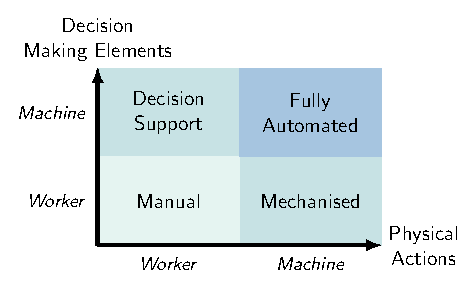
\includegraphics[width=0.5\textwidth]{Diagrams/LoADiagram.pdf}
    \caption{Interpretation of Frohm's Levels of Automation \citep{Frohm2008LevelsManufacturing}}
    \label{fig:LoA}
\end{figure}

None of the reviewed processes achieve full automation, as human input is still required at some level. Mechanisation (the automation of physical tasks), such as the actuation of tooling and of the sheet can be achieved using off-the-shelf industrial robot arms or bespoke machinery. Generally, this enables processes to execute physical tasks to the same, if not greater degree of flexibility, capability and accuracy than the manual counterpart process. Automation of decision-making elements, principally strategy generation, is less straightforward and represents the main challenge facing process designers. For reviewed and applicable processes, a summary outlining three characteristics used to generate and regulate forming strategy is shown in Table \ref{tab:MechProcesses}. For comparison, manual techniques are also listed, using information collected in Section \ref{sec:Manual}.

The strategy generation characteristic outlines the logic used to define and regulate forming strategy for a desired part. A predetermined strategy indicates a strategy that is explicitly defined by an operator, whereas a rule-based strategy is one where the strategy is generated from a set of formulae. In the parentheses, the system is specified further.   The feedback sensors characteristic shows if information is collected and fed back into the system to update the forming strategy in real time. Three categories of data types are listed and if no sensors are installed, then the process is considered open loop --- see \cite{Polyblank2014Closed-loopProspectus}.      

The underlying knowledge/data that forms the basis of the control logic used in a process is also listed. These are arranged into five categories: Analytical --- when the underlying logic is derived from a purely theoretical standpoint, for example a mathematical model; FE --- when the underlying logic uses data generated from finite element simulations; Experimental --- when the underlying logic relies on a series of systematic physical experiments; Heuristic --- when the underlying logic used is based off a rational understanding of the traditional technique;  Smith --- when the underlying logic uses data explicitly captured from experienced smith carrying out the manual process.

Table \ref{tab:MechProcesses} demonstrates the range of different approaches taken to tackle the problem of autonomous strategy generation and regulation of processes. Further discussion on the capabilities of these methods is can be found in section \ref{sec:discussion}. One conclusion that can be drawn, which motivates the proceeding section of this paper is the under-utilisation  of the traditional smith. As none of the automated adaptations of manual techniques used by the traditional smith are yet as versatile their manual counterpart, this implies that large amounts of knowledge, gained through years of experience are being discarded by not capturing, recording and understanding the smith’s craft. Capturing and understanding these skilled actions is challenging due to the tacit nature of the processes and creative approaches are needed to overcome this challenge.

\renewcommand{\arraystretch}{1.2} 
\begin{table}[h] 
    \centering
    \resizebox{\linewidth}{!}{
        


\rowcolors{1}{}{gray!10}
\begin{tabular}{rlcccccccc} \toprule
\rowcolor{white}
                                                                                                         & \multicolumn{1}{c}{\multirow{2}{*}{Strategy Generation}}             & \multicolumn{3}{c}{Feedback Sensors}    & \multicolumn{5}{c}{Control data   context/source}                 \\
\cmidrule(lr){3-5}\cmidrule(lr){6-10}
\rowcolor{white}
                                                                                                                 &                  & Visual         & Force        & Audio       & Analytical   & FE Simulation & Experimental & Heuristic & Smith        \\
\midrule
\textbf{Hammer}                                                                                                                      &                                       &   &   &   &   &   &   &   &   \\
-                                                                                                                           & Manual                                & \checkmark & \checkmark & \checkmark &   &   &   & \checkmark & \checkmark \\
\citep{Ilangovan2016FixturelessForming}                                                                                     & Rule Based (Mechatroforming)          & \checkmark & \checkmark &   &   & \checkmark & \checkmark & \checkmark & \checkmark \\
\citep{Tanaka2005DevelopmentWorking,Tanaka2012DevelopmentSystem,Asakawa2010DevelopmentProcess,Takasugi2012DevelopmentShape} & Rule Based (Novel Analytical)         &   &   &   & \checkmark &   &   & \checkmark &   \\
\citep{Mori1996DeterminationAlgorithm}                                                                                      & Rule Based (Optimise Empirical Model) &   &   &   & \checkmark & \checkmark & \checkmark & \checkmark &   \\
\citep{Mori1998IncrementalDatabase}                                                                                         & Rule Based (Database \& Novel Analytical)                 & \checkmark    &   &   & \checkmark & & \checkmark & \checkmark &   \\
\citep{Tanaka2008FormingMeasurement,Tanaka2014DevelopmentHammering}                                                         & Rule Based (Novel Analytical)         & \checkmark &   &   & \checkmark &   &   & \checkmark &   \\
\citep{Schafer2005IncrementalRobots,Wang2017IncrementalPath,Zhu2019ToolForming,Luo2010ASimulation}                          & Rule Based (Novel Analytical)         &   &   &   & \checkmark &   &   &   &   \\
\textbf{Kraftformer}                                                                                                                 &                                       & \checkmark & \checkmark &   &   &   &   & \checkmark & \checkmark \\
-                                                                                                                           & Manual                                &   &   &   &   &   &   & \checkmark & \checkmark \\
\citep{Scherer2010DrivingProducts}                                                                                          & Manual (Assisted)                     & \checkmark &   &   &   &   &   & \checkmark & \checkmark \\
\citep{Hoffman2009AnHandling}                                                                                               & Predetermined (Reproduce strategy)    &   &   &   &   &   &   & \checkmark & \checkmark \\
\citep{Opritescu2012AutomatedStrategy,Opritescu2016VariationVariance,Hartmann2019Knowledge-basedPartitioning}               & Rule Based (Scale known strategies)   &   &   &   & \checkmark &   & \checkmark & \checkmark &   \\
\citep{Yang2011GeometricalProcess,Yang2009AutomatisierungProgramming}                                                       & Rule Based (Novel Analytical)         &   &   &   & \checkmark &   &   & \checkmark &   \\
\citep{Scherer2013MethodenBlechumformung}                                                                                   & Rule Based (Novel Analytical)         &   &   &   &   & \checkmark &   & \checkmark &   \\
\citep{Opritescu2015AutomatedApproach,Hartmann2019AnFree-forming}                                                           & Rule Based (Neural Network)           &   &   &   &   &   & \checkmark & \checkmark &   \\
\textbf{English   Wheel}                                                                                                             &                                       &   &   &   &   &   &   &   &   \\
-                                                                                                                           & Manual                                & \checkmark & \checkmark &   &   &   &   & \checkmark & \checkmark \\
\citep{Vazquez2017RoboticWheeling}                                                                                          & Rule Based (Novel Analytical)         &   &   &   & \checkmark &   &   & \checkmark &   \\
\citep{Rossi2018ModellingWheel,   Rossi2018Re/LearningSurfaces}                                                             & Rule Based (Neural Network)           &   &   &   &   &   & \checkmark & \checkmark &   \\
\textbf{Spinning}                                                                                                                            &                                       &   &   &   &   &   &   &   &   \\
-                                                                                                                           & Manual                                & \checkmark & \checkmark & \checkmark &   &   &   & \checkmark & \checkmark \\
\citep{Wong2003AProcesses}                                                                                                  & Predetermined (CNC)                   &   &   &   &   &   &   & \checkmark &   \\
\citep{Lloyd1986AnProspective}                                                                                              & Predetermined (PNC)                   &   &   &   &   &   &   & \checkmark & \checkmark \\
\citep{Nzahumunyurwa2001OptimizationProcess}                                                                                & Rule Based (Novel Analytical)         &   &   &   & \checkmark &   &   & \checkmark &   \\
\citep{Hanafi2003VisualSpinning}                                                                                            & Rule Based (Novel Analytical)         & \checkmark &   &   & \checkmark &   &   & \checkmark &   \\
\citep{Auer2004ComparisonSpinning,Henkenjohann2005AnProcess}                                                                & Rule Based (Optimise Empirical Model) &   &   &   & \checkmark &   & \checkmark & \checkmark &   \\
\citep{Polyblank2015TheSpinning}                                                                                            & Rule Based (Novel Analytical)         & \checkmark &   &   & \checkmark & \checkmark &   & \checkmark &   \\
\citep{Arai2006Force-controlledMotors}                                                                                      & Rule Based (Novel Analytical)         &   & \checkmark &   & \checkmark &   & \checkmark & \checkmark &   \\
\bottomrule			   
\end{tabular}
        }
    \caption{Summary of control characteristics used in attempting to automate decision-making elements  in processes derived from metal smithing}
    \label{tab:MechProcesses}
\end{table}

%Table \ref{tab:MechProcesses} shows a number of different approaches taken in an effort to tackle the problem of autonomous strategy generation to control and regulate processes. Using predetermined strategies, significant human input is still required and part shapes are limited. However, as demonstrated by the industrial uptake in PNC spinning (\citep{Lloyd1986AnProspective}), these methods enable repeatable, complex parts to be made, something not yet achieved by rule based systems.

%A number of rule based systems are used to generate and regulate manufacturing strategy, with various forms of underlying logic used to formulate the system. Systems that rely on analytical models are constrained by the requirement for highly detailed models to successfully approximate deformation, as previously alluded to in the literature \citep{Allwood2016Closed-loopForming}. Increasing the degrees of approximation (by using numerical methods for example) results in increased computational time, making it an infeasible method for strategy generation.

%Most frequently, experimental data is used in rule based systems. By physically forming sheets, the nonlinear behaviour of the sheet deformation is captured without need for complex modelling or high power computation. Both the interpolation and extrapolation of this data is done using various methods, one of which being neural networks which can successfully interpret the non-linear nature of deformation. This, along with other experimentally based rule based systems do require collecting large amounts of data to be effective.

%One underutilised source is the traditional smith. As none of the automated adaptations of manual techniques used by the traditional smith are yet as versatile their manual counterpart, this implies that large amounts of knowledge, gained through years of experience are being discarded by not capturing, recording and understanding the smith’s craft. Understanding and capturing these skilled actions is challenging due to the tacit nature of the processes and creative approaches are needed to overcome this challenge.





%Though all these processes strive toward full autonomy, none achieve this as worker input is still required at some level. Comparing processes autonomy is not straightforward as there are many different taxonomies available for ranking the level of autonomy (LoA) of a process \citep{Vagia2015AProposed, Frohm2008LevelsManufacturing}. Here,  Endsley's taxonomy is used \citep{Endsley1999LevelTask} as this specifically focuses on the automation of cognitive tasks (for example crafting) that require real time control \citep{Vagia2015AProposed}. The 10 LoA are shown in table \ref{tab:LoAEndsley}  and are determined by the allocation of four key roles being human (H) or computer (C) controlled.

%\begin{table}[h] 
  %  \centering
    %    \begin{tabular}{clcccc} \toprule
        &                               & \multicolumn{4}{c}{Roles}                                                            \\
\cmidrule(lr){3-6}
\multicolumn{2}{c}{Level of Automation} & \begin{tabular}[c]{@{}c@{}}Monitoring \\ System\end{tabular} & \begin{tabular}[c]{@{}c@{}}Generating \\ Strategy\end{tabular} & \begin{tabular}[c]{@{}c@{}}Selecting \\ Strategy\end{tabular} & \begin{tabular}[c]{@{}c@{}}Implementing \\ Strategy\end{tabular} \\
\cmidrule(lr){1-6}
1       & Manual Control                & H                 & H                   & H                  & H                     \\
2       & Action Support                & H/C               & H                   & H                  & H/C                   \\
3       & Batch Processing              & H/C               & H                   & H                  & C                     \\
4       & Shared Control                & H/C               & H/C                 & H                  & H/C                   \\
5       & Decision Support              & H/C               & H/C                 & H                  & C                     \\
6       & Blended Decision Making       & H/C               & H/C                 & H/C                & C                     \\
7       & Rigid System                  & H/C               & C                   & H                  & C                     \\
8       & Automated Decision Making     & H/C               & H/C                 & C                  & C                     \\
9       & Supervisory Control           & H/C               & C                   & C                  & C                     \\
10      & Full Automation               & C                 & C                   & C                  & C                    \\
\bottomrule
\end{tabular} 
    %\caption{Endsley's Level of Automation \citep{Endsley1999LevelTask}}
    %\label{tab:LoAEndsley}
%\end{table}





%Universal part production, akin to the skilled craftsman in their workshop has not yet been achieved, with most automated processes still requiring substantial human input on some level. Furthermore, with process combination not yet trialled, the individual deformation mechanics of each technique limit the levels of geometric variability achievable by each process. Here we review processes that are inspired by, or use traditional tooling/techniques to form parts and consider the hardware and control techniques used to automate production.

% Differences between experimental and craftsman
% Predetermined and rule based

%[I think it is worth discussing what we're trying to say in this section before we go any further and to also include any mechanised spinning processes. I think it is important to emphasise that most control systems now look to use closed loop control and database/ANN systems to account for the nonlinear behaviour observed in metalforming. This leads onto the next section, that these databases and NNs can be populated/trained through capturing data from skilled craftsmen. I think it would be good to also refer back to fig 22 in \citep{Allwood2016}]

%Nonetheless, a useful starting point is to list and contrast these processes. This allows for comparison of the underlying techniques, methods, sensors and mechanical characteristics for these processes. This allows us to both identify trends and identify useful technologies that might be cross compatible. Table \ref{tab:Process}, summarises applicable processes from section \ref{sec:MechanisedProcess} and summarises the different mechanical components and configurations that can be used to physically manipulate and actuate material as well as various different control strategies to regulate the process. For comparative purposes, the manual counterparts are also listed, using information collected in section \ref{sec:Manual}. 

%Assessing and comparing the merits of these different configurations would be challenging as there is no straightforward way to assess the autonomy of each mechanised variety. However using a previously mentioned classification by Frohm [ref], none of these processes are yet as versatile or efficient as their manual counterpart, so cannot be classified as fully autonomous. EGL: I wasn't sure what you were trying to say here. They are clearly not autonomous since they need human input. Also, what do you mean by merits here? Isn't the idea to look at the underlying techniques/methods/sensors/mechanical characteristics? Isn't that what the table is about? 


%The ultimate goal of autonomous flexible metal forming is 
%Though these processes strive toward a fully autonomous system, none of these achieve full autonomy as they still require worker input at some level. Assessing the merits of the different configurations used in attempting to achieve autonomy, there is no straightforward way of ranking which configurations/components are best.

% LoA - from Endsley
% Flexibility - 

% Flexibility
%		Low - Only a set number of shapes can be formed
%		Med - A small range of interpolated shapes can be formed (possibly in 1D/2D)
%		High - The full range of part shapes achievable by the manual counterpart process can be formed
% Degree of Approximation 

% Analogy with the skilled craftsman(?)
%		Novice - Repeating known actions to achieve known shapes
%		Apprentice - Has some understanding of the system and can define a strategy for forming a range of shapes
%		Expert - Has very good understanding of the system and can define a strategy for forming a greater range of shapes and also adapts this strategy instinctively if needed  

\newpage
\section{Learning from Craftsmen} \label{sec:Learning}

In this section, methods of capturing and utilising the skilled actions of smith are reviewed. The limited set of such activities in the metal forming literature prompts us to consider other domains, revealing the state of the art in this area and hinting at future possibilities. 

\subsection{Learning from the community \label{sec:LfC}}
Despite a decline in professional craftsmen, the art of manual metal smithing is kept alive by an active community of artisans, circulating a wealth of knowledge through a range of widely accessible resources. Though useful to the hobbyist or apprentice, these resources are often overlooked by the academic community as the content lacks in technical understanding and explicitly defined process capabilities. Nevertheless, they can provide a useful starting point for describing techniques used to form shapes, advise on correct machine/tool configurations and give useful tips on how to avoid common mistakes the inexperienced workman or newly commissioned technology might face.

There are a number of written manuals aimed at training apprentice metal smith and hobbyists alike. Some of these manuals, such as Barr's \emph{Sheet Metal Fabrication} series \citep{Barr2013ProfessionalFabrication,Barr2019SheetProjects} detail step-by-step instructions for creating specific parts allowing other similar parts to be made by replicating procedures and slightly adjusting techniques. Other manuals, such as Timings \citep{Timings2008SheetMetalwork}, Thompson \citep{Thompson2007ManufacturingProfessionals} and Wakeford \citep{Wakeford1985SheetWork} take a broader approach by detailing information about individual tools and techniques that can be used to create part shapes. Coppersmithing \citep{Fuller1904ArtForms} and silversmithing \citep{Hill2014ManufacturingProcesses} manuals provide details on similar techniques used to form those materials. There also exist manuals focusing on the operation of a specific tool, such as the English wheel \citep{Longyard2014LearningWheel} and spinning lathe \citep{Tuells1912MetalUsed}, which reflect the complexity of operating these tools.

Despite the thoroughness of these manuals, craftsmen often struggle to articulate the necessary tacit skills required for successful crafting \citep{Wood2009ACraftsmen}. This makes relaying information through manuscript challenging. Recorded instructional videos can be preferable as they give the smith the platform to convey the tacit nature of the task by enacting and thus demonstrating the process. Such resources are prevalent amongst a growing online community of smith, allowing them to connect globally to share and record their expertise. Examples of such content are very common and for the interest of our readers, we can cite a few sources of such work such as Ron Corvell's \emph{Hand Metalworking} series \citep{CorvellRonSeries} and \emph{The Secrets of Metal Shaping} by Lazze \citep{LazzeTheShaping}.

Training courses where skilled craftsmen give interactive demonstrations and tutorials on tools and techniques are another excellent, underutilised resource. The authors note that the opportunity to observe a master craftsman at work and emulate their work under their supervision is an excellent route to adopting their good habits and developing an instinct for the relevant processes and materials. An experienced instructor can also indicate the comparative difficulty of different techniques and part geometries. Very often, such comparisons are not obvious to a novice, or even to trained engineers without practical experience. Designers of automated processes have found it beneficial to familiarise themselves with the manual counterpart through attending such courses during the initial stages of process development \citep{Ilangovan2016FixturelessForming}.

\subsection{Learning from Demonstration} \label{sec:LfD} 
Much like the apprentice during the initial stages of their training, knowledge can be gained by observing a trained, skilled operator carrying out the process. Unlike Section \ref{sec:LfC}, here we focus on quantitative data that can be captured from skilled workers and used in the design or control of automated processes.

Systems acquiring new skills from human expert demonstrators using data acquired through sensors is not new, with Learning from Demonstration (LfD)  an already well-established field \citep{Ravichandar2020RecentDemonstration}. 
However typical manufacturing applications within this field focus on more straightforward tasks such as robotic assembly \citep{Zhu2018RobotSurvey}. Despite this, we look for the various methods and technologies that can be used to capture the actions of the human operator, which are applicable to smithing actions and techniques.

Data can be collected using a vast range of cheap and readily available sensors, and there already exists an extensive review of sensors used to capture different metrics used in industrialised metal forming processes \citep{Allwood2016Closed-loopForming}. Here, we focus on capturing data specific to manual metal smithing processes, extending our search beyond the domain of metal forming. The design activity pattern in Figure \ref{fig:DAP} provides a useful starting point to identify the types of data that are critical to traditional forming and that should be captured. These include parameters that the smith controls: the trajectory of the tools and sheet, the machine configuration and also consider what the smith might be responding to: feedback from both the tool and workpiece in different manifestations --- visual feedback, force feedback etc. 

\subsubsection{Capturing Geometry and Trajectories}
The trajectory and position of both the sheet and tool are key elements of the manufacturing strategy. The geometry of the sheet is also paramount, as during most metal smithing operations, this is the primary desired characteristic of the formed part. Capturing the relative tool positions and sheet geometry is therefore vital to understand the smith’s manufacturing strategy.

Most processes reviewed in Section \ref{sec:Mechanised} make use of some form of technology to capture the geometry of the sheet. These are used either post process to analyse the final form of the sheet, or during the process as an integrated element of the control system. As demonstrated in the aforementioned review by \cite{Allwood2016Closed-loopForming}, there are a vast array of sensors and methods that can be used to capture this type of data. For a given process the required sensing method will be selected based on factors such as resolution, processing time, availability and cost. 

There are fewer examples of technologies and methods used to capture the movement of the metal smith and their tools during manual processing. One example is the Mechatroforming approach, where the trajectory of the sheet is tracked as it is manually worked using two vicon T-series cameras with the data collected used to populate the database control system \citep{Ilangovan2016AnForming}. Similarly, the trajectory of a held hammer is tracked when striking the sheet to estimate the impact force on the sheet. The trajectory of the workpiece as it is manually worked is also captured in a number of cognitive driving strategies discussed in Section \ref{sec:MechKraftformer}. 

Looking beyond the field of metal forming, there are a number of technologies and methods capable of tracking human motions, which can be used to subsequently capture tool/sheet trajectories. This is currently a rapidly expanding field, given a recent explosion in computer vision research. Data is collected through either worn sensors or through vision based systems.

Vision based systems collect data from sensors capturing colour (RGB) or a combination of colour and depth (RGBD) \citep{Zhang2019AMethods}. The challenge in using these types sensors lies in processing streams of data to identify movements and actions. Though off-the-shelf technologies are available with this capability built in (e.g. the Microsoft Kinect --- \cite{Shotton2011Real-timeImages}), this can be achieved using generic, all-purpose cameras with data processed using one of the many different methods outlined in a number of comprehensive reviews \citep{Zhang2019AMethods,Beddiar2020Vision-basedSurvey}. Alternatively, wearable technologies, including electromechanical devices that attach to the body and record movements, can be used. Though the processing of data is more straightforward, these technologies are often more expensive and obtrusive than machine vision systems. Nevertheless, there are again a number of comprehensive reviews into the state of the art of this type of technology used in medical \citep{Homayounfar2020WearableChallenges} and sport \citep{Taborri2020SportOverview} applications.

\subsubsection{Capturing Forces (Haptics)}
In most manual forming processes, human operators are in physical contact with the sheet, whether directly with their limbs or indirectly through the tools they wield. In addition to visual information, then, they can also use haptic feedback to adjust and measure their actions. The word \textit{haptic} refers to anything to do with the sense of touch. During manual sheet forming, this haptic feedback might be a result of the evolving stiffness and strength of the workpiece, vibrations from the workpiece or any other mechanical effects. The smith often describe the sensation of feeling the material as it is worked. The response to haptic feedback can be either a conscious change in manufacturing strategy, or a more tacit change in the force applied to deform the workpiece. 

Haptic feedback is a prominent feature in manual spinning. During this process, the contact between the workpiece and the smith is mediated through the stick-shaped tool, which is held by the craftsman under the armpit and used in combination with a fulcrum pin to deform the rotating workpiece --- see Figure \ref{fig:Drawings}(d). This haptic feedback can be used by the smith to gather important information on the workpiece, including thinning of the blank and hardening of the material. Crucially, force and vibration feedback are used to check that the workpiece is fixing itself tightly to the mandrel beneath, and to monitor its tendency to buckle. Though force feedback is used on many different automated spinning machines \citep{Arai2006Force-controlledMotors}, no study known to the authors has attempted to measure these forces during the manual process. 

However, a haptic spinning system which allows a human operator to control the working roller of a CNC spinning lathe, while providing them with force feedback from the workpiece was recently developed \citep{Russo2019HapticSpinning}. The system employs an off-the-shelf force-feedback joystick (known as Phantom Desktop and currently commercialised by 3D Systems Inc.) in combination with loadcells installed on the two main motion axes of the roller. Using this system, the researchers have invited experienced spinning craftsmen and recorded their actions in a series of over 70 experimental trials, making the database freely available \citep{Russo2020ResearchSpinning}. The force data can be used as an alternative or together with the geometrical trajectory to design better toolpaths in spinning. Moreover, oscillations in the data can potentially be used to check whether wrinkling is about to happen. 

Haptic and other similar data have been collected in an effort to begin to automate other manual manufacturing processes that are sensitive to haptic feedback. A mechatronic device developed by Kalt et al is used to measure force, torque and vibration on the tool during a manual polishing of metallic surfaces as well as tracking tool trajectory and feed rates \citep{Kalt2016TowardsOperation}. Similar tools were developed for use in capturing data for manual grinding \citep{Phan2018InstrumentationWorkpiece} and wood planing \citep{Montebelli2015OnTasks}.


\subsubsection{Capturing Machine Configuration} \label{sec:capturingmachineconfig}
During forming, the smith regularly changes tools and adjusts the machine configuration --- for example changing forming tool during spinning or lower tool pressure when wheeling. Despite this, in most automated sheet forming applications, only one machine set up is considered, possibly to reduce complexity. However, as different machine configurations are often manipulated by craftsmen during the manual process, these must be considered as key elements in the manufacturing strategy.

Capturing the different machine configurations used during  manual smithing is straightforward as these changes are often either visible --- such as tool changes, or measurable --- such as changing lower anvil height when wheeling. However, the authors could find no examples of tracking these configurations during manual processing. Beyond metal forming Manorathna gives a prominent example of how manipulating machine parameters can be used to control the manufacturing process by tracking various parameters for expert and novice welders when working \citep{Manorathna2017HumanAutomation}. 

Though not explicitly learning from the smith, systematic investigations can be carried out to examine the effects of different machine configurations on part deformation. For spinning, a number of process parameters have been investigated, a few examples include spindle speed \citep{Sugar2016AnalysisSteels,Essa2010OptimizationAnalysis}, tool shape \citep{El-Khabeery1991OnCups,Essa2010OptimizationAnalysis} and initial blank properties \citep{Watson2015InvestigationMethod}. Tool shape and wheeling pressure have also been investigated for the English wheel \citep{Bowen2021NumericalProcess}. Furthermore, comprehensive reviews on the influence of process parameters on deformation in incremental sheet forming, a process often associated with the metal smith processes \citep{Music2012TheTools}, suggest the influence of process configuration on deformation \citep{Gatea2016ReviewForming,Gohil2021ReviewProcess}.

\subsubsection{Learning from collected data}
Though data can be collected using a variety of cheap and readily available sensors, designers who are often not skilled craftsmen might not have the ability to interpret this data --- that is to say, how are they to evaluate a good technique/set of data from a bad one, when they themselves are not experts? 
%Furthermore, additional challenges exist in collating data types to be used harmoniously. 
This challenge of eliciting techniques and knowledge from data acquired from skilled craftsmen is not limited to metal forming and there are different groups investigating how similar tacit knowledge can be understood and used.

A straightforward method of identifying skilled techniques is by analysing and comparing the actions of skilled and unskilled craftsmen carrying out identical tasks. Ikemoto studies the manufacturing strategies of five expert and five non-expert craftsmen repairing identically damaged car panel, using only a hammer.  Alongside completing the job to a higher standard, patterns emerge amongst experts for different metrics that are recorded, including strike positions \citep{Ikemoto2018ProcessRepair} and the time spent on tasks \citep{Ikemoto2016ARepair}. This begins to highlight the skilled actions of the expert craftsmen gained over years of experience that can be utilised in automated processes. Similar studies comparing skilled and novice workers have been undertaken for other manual manufacturing processes including machine configurations in welding processes \citep{Manorathna2017HumanAutomation}, stroke directions in both hand lay-up of glass fibre reinforced composites \citep{Xie2016EffectMethod, Kikuchi2016ResearchLay-up} and biometric data (joint angles) during traditional stone knapping \citep{Rein2014MovementTraditions}. 

Having identified a skilled cohort, knowledge can be gained from identifying techniques and patterns that are repeated. An early example of this, is the identification of 15 commonly used gripping techniques used by skilled machinists to grasp objects \citep{Cutkosky1986ModellingHands} which is still widely used for the design of robot arm grippers \citep{Feix2016TheTypes}. This technique of analysing the actions of a skilled cohort has been used to identify seven empirical rules for spinning, such as using both forward and backward passes and maintaining tool speed within a range \citep{Russo2020ResearchSpinning}.
Although the material system is substantially different, similar methods are used to identify techniques in manually layering pre-impregnated woven materials, using data collected from video analysis \citep{Elkington2015HandProcess, Elkington2015StudyingLayup} and later from quantitative movement tracking \citep{Prabhu2017DigitisationTechnology}. From this, new automated processes can be developed \citep{Elkington2016AutomatedMoulds}.

%There are a few notable cases where LfD has been used to control systems, where data has specifically been gathered from skilled craftsmen. Using force and positional data, toolpaths for automated production, using data collected from experts \citep{Ng2017CapturingGrinding}. [need to expand on this and can we find any more examples?]


% - - - - - - - - - - - - - - - - - - - - - - - - - - - - - - - - - - - - - - - - %
% Here I have included some other ref's which might fit in somewhere, but I am not sure where.
% \citep{Lamkull2009} - simulation of human movement. [still not sure how this one fits in exactly?]
% In \citep{Phan2020} a practical approach to estimate human joint stiffness during tooling tasks for the purpose of programming a robot by demonstration.


\section{Discussion}\label{sec:discussion}

Below, we distil and respond to three key questions that emerge from the reviewed literature. This allows us to highlight new opportunities and challenges in this area and elaborate on the current state of the art.

\newcommand{\question}[1]{\vspace{1em} \noindent \textit{#1} \vspace{0.5em}}

\question{1. What tools and techniques are used by the traditional smith and how can they be of use to modern process designers?}

Using a range of tooling and techniques, the smith is capable of forming a variety of parts from initially flat sheets. Having reviewed an array of manual techniques used by smiths in Section \ref{sec:Manual}, a taxonomy of tools and techniques is presented in Figure \ref{fig:ManualTaxonomy}. These are grouped according to the tooling used, with each technique having a unique deformation mechanism and geometric forming capability. However, the ad hoc nature of the manufacturing paradigm implies there are several more processes not included, which include tools not considered in this review --- bead rollers for example. These could serve as a useful starting point for novel process development. A more comprehensive taxonomy could be produced by consulting the many underutilised resources outlined in Section \ref{sec:Learning}.

\begin{figure}[h]
	\centering
    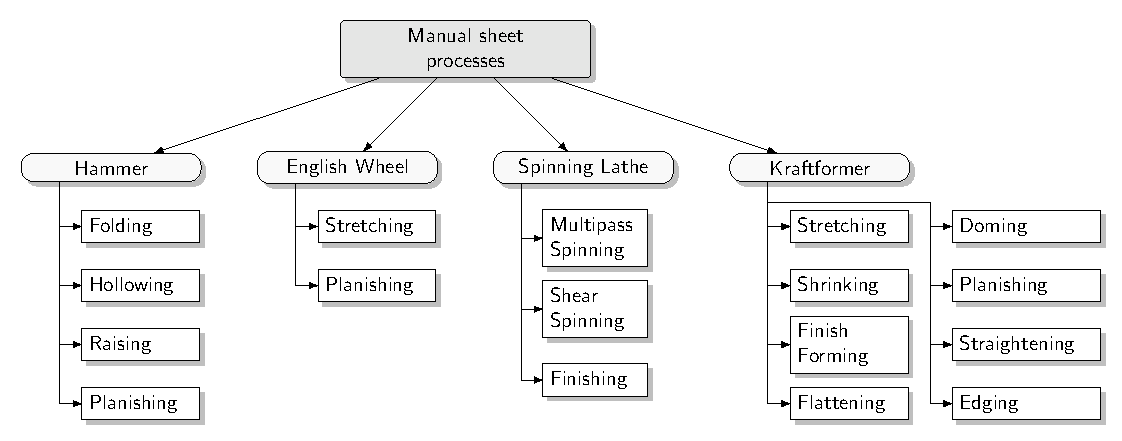
\includegraphics[width=\linewidth]{Diagrams/Taxonomy3.pdf}
    \caption{Taxonomy of manual processes}
    \label{fig:ManualTaxonomy}
\end{figure}

%Many of the techniques listed in the taxonomy remain ambiguous, with both deformation mechanism and specific procedure not yet explicitly defined. A more thorough and quantitative understanding of these traditional techniques could lead to improved capabilities in the operation of automated processes. For example, a better understanding of the stretching technique used in manual wheeling could improve the operation of the reviewed automated wheeling processes \citep{Vazquez2017RoboticWheeling,Rossi2018ModellingWheel}. An improved understanding could also lead to the development of new, novel processes as demonstrated by the fold-shearing \citep{Allwood2019Folding-shearing:Change} and raising by spinning \citep{Russo2020RaisingSpinning} processes, both of which were derived from manual spinning techniques.


%As parts produced by the smith are often made from constituent complex geometries, forming an overall shape often requires multiple operations, utilising different techniques. In previous motorcycle fuel tank example, hollowing is just the first stage of production with raising and wheeling techniques subsequently used to form the shape, alongside other auxiliary processes such as cutting, welding and finishing operations \citep{Barr2013ProfessionalFabrication}. Selection of tooling/technique is part of the smith's tacit logic and is further complicated by process selection variability within manual processing. This is demonstrated in Figure \ref{fig:ShapeDevBow} which outlines the various ways which the smith might form a deep bowl using different tools and techniques. The choice of technique will be based on the smith’s individual skills, past experiences and availability of tools. % why might the smith choose one way over another? (better quality, easier etc..)


Each of the techniques used by the smith will have a unique, constrained range of possible geometries that can be formed from a preformed panel, created in an earlier process. This is why a combination of processes are commonly used when forming parts. It follows that when considering an automated solution for universal part production using processes derived from metal smithing, using multiple tools/techniques will likely be necessary. This would currently be a complex and challenging task as alongside the poor repeatability of individual processes, automated methods for flexible process selection are in their infancy  \citep{Hamouche2018ClassificationLearning}.

Despite inherent challenges, the merits of automating these manual processes remain multifaceted. Each manual technique used by the smith shapes material incrementally and the localised deformation suggests processes are scalable. Unlike many other flexible, incremental processes (ISF for example), none of the smith’s processes reviewed in Section \ref{sec:Manual} require clamping at the boundary of the sheet. This is favourable as this clamping often leads to a build-up of residual stresses and causes springback which limits the forming capabilities of these processes.

\question{2. What approaches can be taken to automate the generation of forming strategy}

Low levels of decision-making automation use mechanised machinery to physically replicate the actions of the worker/smith. Using these systems, decision-making elements are predetermined so part variations are limited to captured strategies. Another limitation of using these methods is the requirement for a skilled smith to initially form the desired part, and specialist equipment to record the forming strategy. Like other open-loop processes, these systems are incapable of adjusting strategy for unexpected deformations in real-time. Nevertheless, these systems have successfully demonstrated part production using a kraftforming machine \citep{Hoffman2009AnHandling} and are commonly used in industrialized spinning \citep{ Lloyd1986AnProspective}. 

Only one example of decision support could be identified. This is when physical tasks are carried out manually and an autonomous system provides guidance on the forming strategy --- see Figure \ref{fig:LoA}. This system uses a heads up display fitted to a kraftformer to allow the worker to check the formed part against the desired shape in real time during manual forming \citep{Scherer2010DrivingProducts}. The nontraditional resources outlined in section \ref{sec:LfC} can provide a similar level of decision support as there are many examples of forming strategies that could be used to create a wide range of parts, using either manual or mechanised tooling.

A number of rule-based methods for generating forming strategy have been developed. Methods that rely on analytically derived models and formulae often cannot capture the complex mechanics associated with the plastic deformation of sheets \citep{Yang2011GeometricalProcess,Yang2009AutomatisierungProgramming,Vazquez2017RoboticWheeling,Polyblank2015TheSpinning} or the range of parts that can be formed are significantly limited \citep{Nzahumunyurwa2001OptimizationProcess}. Some analytical models also rely on user input to select parameters (other than the desired part shape) in the algorithm for determining forming strategy, lowering the level of decision-making autonomy of the process \citep{Tanaka2012DevelopmentSystem,Asakawa2010DevelopmentProcess}.

Numerical methods can be used to more accurately compute deformation for a given strategy \citep{Bowen2021NumericalProcess,Hoffmann2005StudiesMetal}. This provides an insight into the mechanisms of deformation leading to a better understanding of the process capability. However, these models are often computationally expensive and are subsequently infeasible for the generation of manufacturing strategies \citep{Scherer2013MethodenBlechumformung,Polyblank2015TheSpinning}. 

Many rule-based systems rely on data that has been captured experimentally to generate strategies for parts. These methods inherently capture the nonlinear behaviour of the deformation without the need for complex modelling. A database of strategies can be used to select a strategy that produces a part best matching that of the desired part shape \citep{Mori1998IncrementalDatabase}. However, similar to play-back systems, the range of part shapes is limited to captured strategies and part shapes. Instead, different methods have been used to interpolate/extrapolate the captured data, making use of several statistical methods \citep{Opritescu2012AutomatedStrategy,Opritescu2016VariationVariance,Hartmann2019Knowledge-basedPartitioning,Henkenjohann2005AnProcess}. Empirical models have also been developed using collected data, which can be optimised to produce a forming strategy \citep{Mori1996DeterminationAlgorithm,Auer2004ComparisonSpinning}.

More recently, experimental data has been used to train neural networks. Similar to the apprentice smith, these systems learn from past experiences and are highly capable of interpreting non-linear behaviour. However, these systems are often constrained by the vast amounts of data required to effectively train systems. Some of the processes reviewed overcome this by reducing the complexity of parts formed \citep{Opritescu2015AutomatedApproach}, augmenting data \citep{Rossi2018ModellingWheel,Rossi2018Re/LearningSurfaces} or by sufficiently tuning the network and pre-processing the data \citep{Hartmann2019AnFree-forming}.

Some processes use integrated sensors to feedback data into the control system. These adjust strategy to account for stochastic variations between sheets or to account for inaccuracies in the control logic which can result in unforeseen deformations. Reviewing the logic underlying the smith’s manual process (Section \ref{sec:tacitknowledge}) reveals that smiths are highly cognisant during crafting and make use of many different forms of feedback in regulating the strategy. In contrast to the manual smith, only a few automated processes include sensors into the system to regulate the process. 

The geometry of the part during forming is the most common source of feedback data captured to adjust the strategy. A number of processes collect data at regular intervals or continuously throughout processing \citep{Mori1998IncrementalDatabase,Ilangovan2016AnForming,Tanaka2008FormingMeasurement,Tanaka2014DevelopmentHammering}. This enables online adjustment of forming strategy to reduce part errors. Some spinning processes use force feedback as the primary element of the forming strategy. By setting the tool to exert a constant force against a shaped and mounted mandrel this enables autonomous forming of parts, including asymmetric parts \citep{Arai2006Force-controlledMotors}. However, both the mandrel and forming force require mounting and setting respectively. One method of feedback not yet used in automated processes is the use of audio cues, despite this being a key indication of the onset of wrinkling in manual spinning.

\question{3. How can new, automated processes be created or improved by observing the skilled smith?}

Many of the reviewed processes make use of a heuristic understanding of the smith’s techniques when designing new processes. However, there are only a few examples of process designers observing the intricate, skilled actions of the smith that enable such versatile manufacturing. Closer observation of the smith’s manual techniques can benefit both the design and the operation of modern, automated processes in many ways.

Observing the smith and gaining a more complete understanding of the range of traditional techniques they use could lead to the development of new, novel processes with improved forming capabilities. Only a few of the manual techniques listed in the partial taxonomy --- shown in Figure \ref{fig:ManualTaxonomy} --- have received attention from modern-day process designers, presenting a significant research opportunity. A better understanding of traditional techniques could also improve the operation of readily established processes. For example, a traditional stretching technique can be utilized during the operation of the reviewed automated wheeling processes \citep{Vazquez2017RoboticWheeling,Rossi2018ModellingWheel}. 
Furthermore, this could lead to the development of new processes through reinvented tooling, similar to the folding-shearing \citep{Allwood2019Folding-shearing:Change} and the raising by spinning \citep{Russo2020RaisingSpinning} processes.

Often, automated processes utilise only a limited subset of machine parameters as part of the forming strategy in comparison to manual processes. Numerous studies have demonstrated the effect these parameters such as tool shape or forming pressure can have on deformation --- see Section \ref{sec:capturingmachineconfig}. This implies that including these process parameters as variables in the forming strategy could extend the capabilities of current processes. However, additional control parameters result in adding complexity to an already complex system. This can be simplified by observing and comparing the strategies of skilled and unskilled smiths and identifying key, influential process parameters used by skilled smith to successfully form parts. Such comparisons have been made for the skilled tasks of repairing of panels \citep{Ikemoto2016ARepair} and welding \citep{Manorathna2017HumanAutomation}.

The domain of learning from demonstration provides a range of examples of systems learning from skilled operators. However, the tacit nature of these traditional processes makes this a more challenging task. Nevertheless, processes have been controlled using data collected from skilled smith \citep{Ilangovan2016AnForming} or from systematic experiments \citep{Ilangovan2016FixturelessForming,Mori1996DeterminationAlgorithm, Mori1998IncrementalDatabase,Opritescu2012AutomatedStrategy,Opritescu2016VariationVariance,Hartmann2019Knowledge-basedPartitioning,Opritescu2015AutomatedApproach,Hartmann2019AnFree-forming,Rossi2018ModellingWheel, Rossi2018Re/LearningSurfaces,Auer2004ComparisonSpinning,Henkenjohann2005AnProcess,Arai2006Force-controlledMotors}, suggesting LfD methods are feasible.

One possible reason these methods are not more commonly used could be the limited access to technologies used to capture data from the smith.  Figure \ref{fig:DAP} provides an insight into the data streams which enable the smith to successfully form parts and Section \ref{sec:tacitknowledge} outlines the importance of this feedback data. Solutions for capturing such data can be found by looking beyond the metal forming sector, specifically the gaming, medical and sport sectors where there are many different technologies that could provide solutions for capturing the actions of the smith.

This collected data could be used to not necessarily directly control the process, but can be used to inform process designers. For example, seven rules of spinning are defined from analysing collected data which can be used in the development of automated manufacturing strategies \citep{Russo2021SevenSpinning}. Similarly, identifying regular patterns in the strategies of skilled workers both quantitatively \citep{Kalt2016TowardsOperation,Phan2018InstrumentationWorkpiece} or qualitatively \citep{Cutkosky1986ModellingHands,Elkington2015HandProcess} can be used to identify techniques used by skilled craftsmen. This could be used to identify a range of forming strategies that can be used to successfully form parts.


 % EGL: I wonder if we should comments how all these processes are essentially thinning/stretching or thickening/compressing the sheet locally and we worry about the same failures in all of them (wrinkling, tearing). We can also say that because in all cases we have free boundaries, springback and residual stresses (common challenges with many modern processes) is less of an issue.
 
 %1 - There are many different traditional crafting processes.
%There is no taxonomy of processes
%The art of smithing is potentially being lost

%2 - In mechanised variant's the specific techniques are often overlooked - hammering is a prime example.
%Furthermore, there is no integration of processes to form an overall shape.
 
%3 -  Mechanised variant's are viable
%A very limited subset of process parameters and sensing are usually included in these invented processes. 
%Given the advances in technology, the process of physical mechanisation is straightforward. 


%\begin{enumerate}

%\item A lot of the panel beater's processes are ad hoc and/or not clearly defined. As well as scope for defining a more rigorous taxonomy, this also implies there are several opportunities to develop new techniques through closer observation of these craftsman.
%\item To achieve a system that is as versatile/flexible as the smith, a combination of processes will likely be needed. This will be challenging until individual processes have been fully established.
%\item With the decline in traditional smiths, the `art' of crafting (knowledge base of techniques and processes) is in danger of being lost. Establishing mechanised processes preserves these.
%\item There are technologies (sensors, control strategies) that have been used in some mechanised processes that could be applicable to other processes
%\item As mechanised processes are not yet as versatile as their manual counterpart, there is still a lot we can learn. This can be done using some of the many sensors used in the domain of LfD.
%\item The similarities between NNs and the craftsman, with regards the way they both learn through experience. 
%\item Database/ ANN approaches provide a method that can be populated by different data. For example, FE and human skill capture is used to inform the mechatroforming approach. These are useful as increasing computational powers should bring about more data rich simulations which could be used to populate databases in a cost effective manner.]
%\item The studies in \ref{tab:MechProcesses} support the earlier argument [what earlier arguement?] that a very limited subset of process parameters and sensing are usually included in these invented processes. Only a small subset of parameters are also trialled (forming force, tool shape etc)

%\end{enumerate}

% [Comment on trends - Work carried out in section \ref{sec:tacitknowledge} demonstrated one of the key enabling characteristics of the craftsman is that they are very cognisant, making use of the different senses . This is reflected in the manual processes by the craftsman using many different senses to...]

\section{Conclusion}

A paradigm shift towards personalised production has brought about the requirement for new, flexible sheet metal forming processes, capable of efficiently forming an extended range of geometries without the need for bespoke tooling. As the traditional metal smith possesses such versatility, techniques used by the smith have provided a useful starting point for novel process development.  This paper has identified and analysed four processes and a number of associated manual techniques commonly used by the smith. A taxonomy of manual processes is assembled, but remains incomplete, pending further investigation into the other tools/techniques used by the smith. Alongside this, the smith’s cognitive process was investigated and a model is constructed which identifies the information channels that require monitoring for successful automation of the manual processes.

Automated processes which are derived from, or are analogous to techniques used by the smith are reviewed and grouped together by tooling. These processes either take advantage of the extended forming capabilities of traditional techniques by replicating the deformation mechanism using reinvented tooling or use traditional tooling, with various physical and decision-making elements automated. 

The control characteristics used to automate decision-making elements in processes derived from metal smithing were summarised. It was found that most of the attempts made so far were heuristic, while only very few studies attempted to learn directly from the smiths. Given their wealth of experience, we reviewed ways in which process design could learn from smiths. Two main methods of learning from the smith were identified: learning from the community and learning from demonstration. The former provides a wealth of knowledge that is overlooked by the academic community which can provide a better understanding of the tacit techniques used by the smith. The latter provides a number of established methods/technologies from other domains. These allow data to be captured from the smith performing the manual process to enhance the design and operation of new, automated processes.



\section*{Acknowledgements}
DTB is funded by an EPSRC studentship while both DTB and EGL benefited from a Faculty of Engineering \& Design starter fund generously provided by the University of Bath. 


%%References
\renewcommand{\bibname}{References}
%%Changes Bibliography to read References
\clearpage
%\bibliographystyle{agsm}
%\bibliographystyle{unsrt}
\bibliographystyle{apa-good}
%\bibliographystyle{ksfh_nat}
%%%% THIS IS WHERE YOU NEED TO EXPORT MENDLE TO %%%%
\bibliography{references}
%%%% THIS IS WHERE YOU NEED TO EXPORT MENDLE TO %%%%

%\end{multicols}
\end{document}